\chapter{Adversarial search}\label{chap:5}
\section{Go}
Go is a two-player strategic board game that originated in China, where it has been played for at least \num{2500} years, but is also very popular in East Asia; only in recent years it has spread to the rest of the world as well. It is a strategically very complex game despite its simple rules; a Korean proverb says that ``no game of go has ever been played twice'', which is likely if you consider that there are approximately $\num{2.08e170}$ different possible positions.

The word Go is a short form of the Japanese word \emph{igo} (\begin{CJK}{UTF8}{min}囲碁\end{CJK}), literally ``encirclement board game'' or ``board game of surrounding''. In fact the Go is played by two players who alternately place black and white pawns, called \emph{stones}, on the vacant intersections of a board formed by a $19\times19$ grid (Fig.~\ref{Go}), called \emph{goban} (\begin{CJK}{UTF8}{min}碁盤\end{CJK}). The usual board size is a $19\times19$ grid but for beginners, or for playing quick games, the smaller board sizes of $13\times13$ and $9\times9$ are also popular. The aim of the game is to control an area of the game greater than that controlled by the opponent; for this purpose the players try to arrange their stones so that they cannot be captured, at the same time carving out territories that the opponent cannot invade without being captured. See \url{https://en.wikipedia.org/wiki/Rules_of_Go} for the complete list of rules.
\begin{figure}[h!t]
\centering
%\begin{subfigure}[ht]{0.48\textwidth}
%	\centering
%	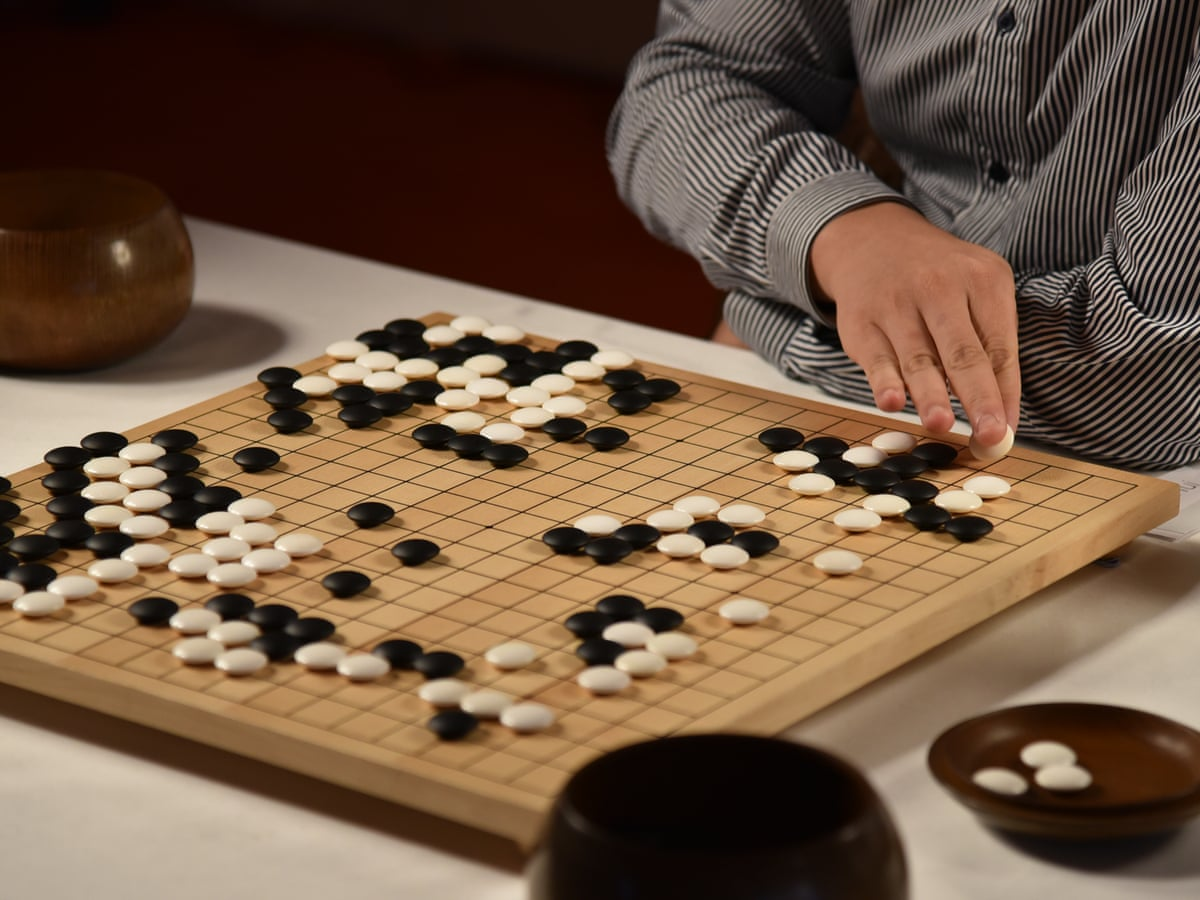
\includegraphics[width=\textwidth]{Go Game (2)}
%	\caption{}\label{Go_Game_(2)}
%\end{subfigure}
%\hfill
\begin{subfigure}[ht]{0.46\textwidth}
	\centering
	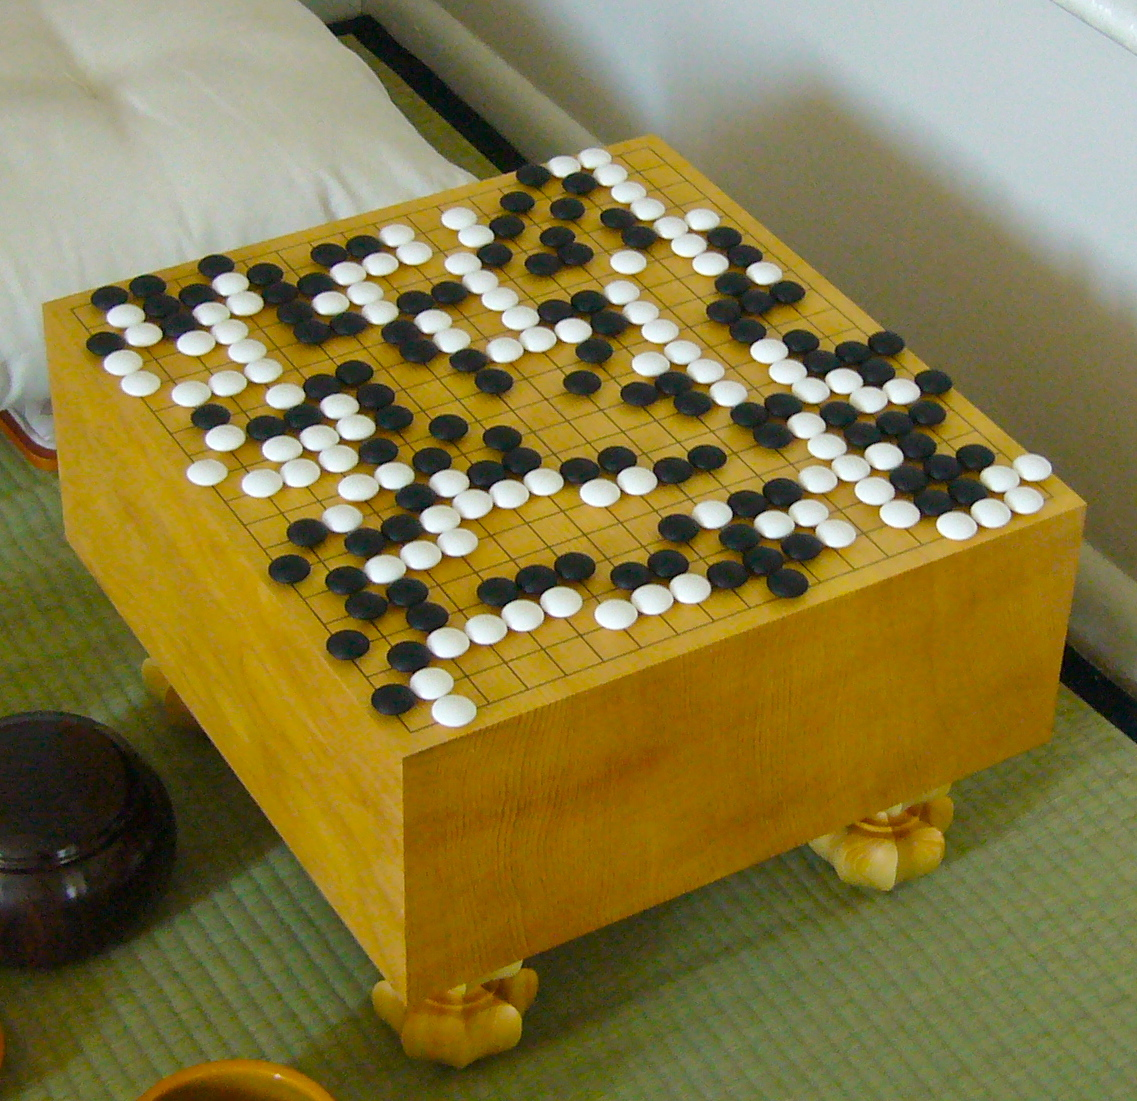
\includegraphics[width=\textwidth]{Floor Goban}
        \caption{The Go board (generally referred to by its Japanese name \emph{goban}, \begin{CJK}{UTF8}{min}碁盤\end{CJK}).}\label{Floor_Goban}
\end{subfigure}
\hfill
\begin{subfigure}[ht]{0.46\textwidth}
	\centering
	%renewcommand only in this environment for the shadows
	\renewcommand\gobstone[3][]{%
		\begin{scope}[shift={(#2,#3)}]
	        	\clip (0,0) circle (0.5);
		        \shade[outer color=black,inner color=black!55] (0,0) ++ (115:0.4) circle (0.5+0.4);
		\end{scope}}
	\renewcommand\gowstone[3][]{%
		\begin{scope}[shift={(#2,#3)}]
	        	\clip (0,0) circle (0.5);
		        \shade[outer color=black!15!white, inner color=white] (0,0) ++ (115:0.4) circle (0.5+0.4);
		\end{scope}}
	\resizebox{\textwidth}{!}{%
	\begin{animateinline}[controls,buttonbg=0.95,buttonsize=4em,poster=last,autopause,timeline=Animation_Go_Game.txt,begin={\begin{tikzpicture}\useasboundingbox (-1,-1) rectangle (19,19);},end={\end{tikzpicture}}]{1.25}
		% #0
		\path[clip,rounded corners=10pt] (-1,-1) rectangle (19,19);
		\node[inner sep=0pt,outer sep=0pt,opacity=0.75] at (9,9) {
\includegraphics[width=20cm,height=20cm]{Wood Texture}};
		\draw[line width=1.2pt] (0,0) rectangle (18,18);
		\foreach \x in {1,...,17} {\draw[] (\x,0) -- (\x,18);}
		\foreach \y in {1,...,17} {\draw[] (0,\y) -- (18,\y);}
		\fill (3,3) circle (0.08);
		\fill (9,3) circle (0.08);
		\fill (15,3) circle (0.08);
		\fill (3,9) circle (0.08);
		\fill (9,9) circle (0.08);
		\fill (15,9) circle (0.08);
		\fill (3,15) circle (0.08);
		\fill (9,15) circle (0.08);
		\fill (15,15) circle (0.08);
		% #1
		\newframe \goshadow{16}{15}
		% #2
		\newframe \goshadow{3}{15}
		% #3
		\newframe \goshadow{15}{2}
		% #4
		\newframe \goshadow{3}{2}
		% #5
		\newframe \goshadow{13}{15}
		% #6
		\newframe \goshadow{15}{4}
		% #7
		\newframe \goshadow{16}{4}
		% #8
		\newframe \goshadow{16}{5}
		% #9
		\newframe \goshadow{16}{3}
		% #10
		\newframe \goshadow{15}{5}
		% #11
		\newframe \goshadow{13}{2}
		% #12
		\newframe \goshadow{15}{9}
		% #13
		\newframe \goshadow{2}{16}
		% #14
		\newframe \goshadow{2}{15}
		% #15
		\newframe \goshadow{3}{16}
		% #16
		\newframe \goshadow{4}{15}
		% #17
		\newframe \goshadow{5}{17}
		% #18
		\newframe \goshadow{2}{8}
		% #19
		\newframe \goshadow{16}{11}
		% #20
		\newframe \goshadow{3}{4}
		% #21
		\newframe \goshadow{6}{9}
		% #22
		\newframe \goshadow{15}{16}
		% #23
		\newframe \goshadow{15}{15}
		% #24
		\newframe \goshadow{14}{16}
		% #25
		\newframe \goshadow{14}{15}
		% #26
		\newframe \goshadow{1}{16}
		% #27
		\newframe \goshadow{1}{17}
		% #28
		\newframe \goshadow{4}{17}
		% #29
		\newframe \goshadow{1}{15}
		% #30
		\newframe \goshadow{4}{16}
		% #31
		\newframe \goshadow{9}{16}
		% #32
		\newframe \goshadow{1}{14}
		% #33
		\newframe \goshadow{0}{16}
		% #34
		\newframe \goshadow{2}{18}
		% #35
		\newframe \goshadow{13}{17}
		% #36
		\newframe \goshadow{12}{16}
		% #37
		\newframe \goshadow{13}{16}
		% #38
		\newframe \goshadow{5}{7}
		% #39
		\newframe \goshadow{7}{9}
		% #40
		\newframe \goshadow{0}{14}
		% #41
		\newframe \goshadow{15}{8}
		% #42
		\newframe \goshadow{14}{8}
		% #43
		\newframe \goshadow{15}{7}
		% #44
		\newframe \goshadow{14}{7}
		% #45
		\newframe \goshadow{16}{9}
		% #46
		\newframe \goshadow{14}{9}
		% #47
		\newframe \goshadow{12}{4}
		% #48
		\newframe \goshadow{12}{5}
		% #49
		\newframe \goshadow{11}{5}
		% #50
		\newframe \goshadow{13}{4}
		% #51
		\newframe \goshadow{11}{4}
		% #52
		\newframe \goshadow{8}{2}
		% #53
		\newframe \goshadow{7}{3}
		% #54
		\newframe \goshadow{8}{3}
		% #55
		\newframe \goshadow{7}{5}
		% #56
		\newframe \goshadow{7}{2}
		% #57
		\newframe \goshadow{15}{10}
		% #58
		\newframe \goshadow{14}{10}
		% #59
		\newframe \goshadow{12}{7}
		% #60
		\newframe \goshadow{12}{6}
		% #61
		\newframe \goshadow{11}{6}
		% #62
		\newframe \goshadow{12}{8}
		% #63
		\newframe \goshadow{14}{11}
		% #64
		\newframe \goshadow{13}{11}
		% #65
		\newframe \goshadow{13}{12}
		% #66
		\newframe \goshadow{12}{11}
		% #67
		\newframe \goshadow{12}{12}
		% #68
		\newframe \goshadow{8}{15}
		% #69
		\newframe \goshadow{9}{15}
		% #70
		\newframe \goshadow{11}{12}
		% #71
		\newframe \goshadow{8}{14}
		% #72
		\newframe \goshadow{7}{14}
		% #73
		\newframe \goshadow{11}{11}
		% #74
		\newframe \goshadow{10}{12}
		% #75
		\newframe \goshadow{12}{9}
		% #76
		\newframe \goshadow{11}{10}
		% #77
		\newframe \goshadow{11}{8}
		% #78
		\newframe \goshadow{13}{7}
		% #79
		\newframe \goshadow{13}{8}
		% #80
		\newframe \goshadow{12}{10}
		% #81
		\newframe \goshadow{6}{3}
		% #82
		\newframe \goshadow{6}{2}
		% #83
		\newframe \goshadow{12}{14}
		% #84
		\newframe \goshadow{8}{13}
		% #85
		\newframe \goshadow{9}{14}
		% #86
		\newframe \goshadow{7}{12}
		% #87
		\newframe \goshadow{2}{3}
		% #88
		\newframe \goshadow{3}{3}
		% #89
		\newframe \goshadow{1}{6}
		% #90
		\newframe \goshadow{2}{5}
		% #91
		\newframe \goshadow{2}{9}
		% #92
		\newframe \goshadow{2}{7}
		% #93
		\newframe \goshadow{1}{5}
		% #94
		\newframe \goshadow{2}{4}
		% #95
		\newframe \goshadow{3}{10}
		% #96
		\newframe \goshadow{10}{7}
		% #97
		\newframe \goshadow{1}{4}
		% #98
		\newframe \goshadow{2}{2}
		% #99
		\newframe \goshadow{1}{9}
		% #100
		\newframe \goshadow{1}{8}
		% #101
		\newframe \goshadow{9}{7}
		% #102
		\newframe \goshadow{6}{8}
		% #103
		\newframe \goshadow{0}{8}
		% #104
		\newframe \goshadow{0}{7}
		% #105
		\newframe \goshadow{5}{9}
		% #106
		\newframe \goshadow{8}{6}
		% #107
		\newframe \goshadow{0}{9}
		% #108
		\newframe \goshadow{1}{7}
		% #109
		\newframe \goshadow{6}{6}
		% #110
		\newframe \goshadow{5}{6}
		% #111
		\newframe \goshadow{6}{7}
		% #112
		\newframe \goshadow{5}{8}
		% #113
		\newframe \goshadow{7}{8}
		% #114
		\newframe \goshadow{10}{8}
		% #115
		\newframe \goshadow{10}{9}
		% #116
		\newframe \goshadow{11}{7}
		% #117
		\newframe \goshadow{5}{5}
		% #118
		\newframe \goshadow{3}{8}
		% #119
		\newframe \goshadow{4}{9}
		% #120
		\newframe \goshadow{15}{3}
		% #121
		\newframe \goshadow{16}{2}
		% #122
		\newframe \goshadow{9}{8}
		% #123
		\newframe \goshadow{9}{9}
		% #124
		\newframe \goshadow{11}{9}
		% #125
		\newframe \goshadow{4}{8}
		% #126
		\newframe \goshadow{11}{14}
		% #127
		\newframe \goshadow{7}{15}
		% #128
		\newframe \goshadow{13}{14}
		% #129
		\newframe \goshadow{13}{13}
		% #130
		\newframe \goshadow{17}{10}
		% #131
		\newframe \goshadow{16}{10}
		% #132
		\newframe \goshadow{6}{15}
		% #133
		\newframe \goshadow{7}{16}
		% #134
		\newframe \goshadow{14}{12}
		% #135
		\newframe \goshadow{15}{11}
		% #136
		\newframe \goshadow{6}{16}
		% #137
		\newframe \goshadow{10}{2}
		% #138
		\newframe \goshadow{7}{17}
		% #139
		\newframe \goshadow{8}{16}
		% #140
		\newframe \goshadow{17}{8}
		% #141
		\newframe \goshadow{17}{7}
		% #142
		\newframe \goshadow{18}{7}
		% #143
		\newframe \goshadow{17}{9}
		% #144
		\newframe \goshadow{16}{16}
		% #145
		\newframe \goshadow{17}{15}
		% #146
		\newframe \goshadow{6}{17}
		% #147
		\newframe \goshadow{11}{15}
		% #148
		\newframe \goshadow{11}{13}
		% #149
		\newframe \goshadow{12}{17}
		% #150
		\newframe \goshadow{13}{3}	%-------------------------------------------------------------------------------------------------------------------------------------------------------------
		% #1
		\newframe \gobstone{16}{15}
		% #2
		\newframe \gowstone{3}{15}
		% #3
		\newframe \gobstone{15}{2}
		% #4
		\newframe \gowstone{3}{2}
		% #5
		\newframe \gobstone{13}{15}
		% #6
		\newframe \gowstone{15}{4}
		% #7
		\newframe \gobstone{16}{4}
		% #8
		\newframe \gowstone{16}{5}
		% #9
		\newframe \gobstone{16}{3}
		% #10
		\newframe \gowstone{15}{5}
		% #11
		\newframe \gobstone{13}{2}
		% #12
		\newframe \gowstone{15}{9}
		% #13
		\newframe \gobstone{2}{16}
		% #14
		\newframe \gowstone{2}{15}
		% #15
		\newframe \gobstone{3}{16}
		% #16
		\newframe \gowstone{4}{15}
		% #17
		\newframe \gobstone{5}{17}
		% #18
		\newframe \gowstone{2}{8}
		% #19
		\newframe \gobstone{16}{11}
		% #20
		\newframe \gowstone{3}{4}
		% #21
		\newframe \gobstone{6}{9}
		% #22
		\newframe \gowstone{15}{16}
		% #23
		\newframe \gobstone{15}{15}
		% #24
		\newframe \gowstone{14}{16}
		% #25
		\newframe \gobstone{14}{15}
		% #26
		\newframe \gowstone{1}{16}
		% #27
		\newframe \gobstone{1}{17}
		% #28
		\newframe \gowstone{4}{17}
		% #29
		\newframe \gobstone{1}{15}
		% #30
		\newframe \gowstone{4}{16}
		% #31
		\newframe \gobstone{9}{16}
		% #32
		\newframe \gowstone{1}{14}
		% #33
		\newframe \gobstone{0}{16}
		% #34
		\newframe \gowstone{2}{18}
		% #35
		\newframe \gobstone{13}{17}
		% #36
		\newframe \gowstone{12}{16}
		% #37
		\newframe \gobstone{13}{16}
		% #38
		\newframe \gowstone{5}{7}
		% #39
		\newframe \gobstone{7}{9}
		% #40
		\newframe \gowstone{0}{14}
		% #41
		\newframe \gobstone{15}{8}
		% #42
		\newframe \gowstone{14}{8}
		% #43
		\newframe \gobstone{15}{7}
		% #44
		\newframe \gowstone{14}{7}
		% #45
		\newframe \gobstone{16}{9}
		% #46
		\newframe \gowstone{14}{9}
		% #47
		\newframe \gobstone{12}{4}
		% #48
		\newframe \gowstone{12}{5}
		% #49
		\newframe \gobstone{11}{5}
		% #50
		\newframe \gowstone{13}{4}
		% #51
		\newframe \gobstone{11}{4}
		% #52
		\newframe \gowstone{8}{2}
		% #53
		\newframe \gobstone{7}{3}
		% #54
		\newframe \gowstone{8}{3}
		% #55
		\newframe \gobstone{7}{5}
		% #56
		\newframe \gowstone{7}{2}
		% #57
		\newframe \gobstone{15}{10}
		% #58
		\newframe \gowstone{14}{10}
		% #59
		\newframe \gobstone{12}{7}
		% #60
		\newframe \gowstone{12}{6}
		% #61
		\newframe \gobstone{11}{6}
		% #62
		\newframe \gowstone{12}{8}
		% #63
		\newframe \gobstone{14}{11}
		% #64
		\newframe \gowstone{13}{11}
		% #65
		\newframe \gobstone{13}{12}
		% #66
		\newframe \gowstone{12}{11}
		% #67
		\newframe \gobstone{12}{12}
		% #68
		\newframe \gowstone{8}{15}
		% #69
		\newframe \gobstone{9}{15}
		% #70
		\newframe \gowstone{11}{12}
		% #71
		\newframe \gobstone{8}{14}
		% #72
		\newframe \gowstone{7}{14}
		% #73
		\newframe \gobstone{11}{11}
		% #74
		\newframe \gowstone{10}{12}
		% #75
		\newframe \gobstone{12}{9}
		% #76
		\newframe \gowstone{11}{10}
		% #77
		\newframe \gobstone{11}{8}
		% #78
		\newframe \gowstone{13}{7}
		% #79
		\newframe \gobstone{13}{8}
		% #80
		\newframe \gowstone{12}{10}
		% #81
		\newframe \gobstone{6}{3}
		% #82
		\newframe \gowstone{6}{2}
		% #83
		\newframe \gobstone{12}{14}
		% #84
		\newframe \gowstone{8}{13}
		% #85
		\newframe \gobstone{9}{14}
		% #86
		\newframe \gowstone{7}{12}
		% #87
		\newframe \gobstone{2}{3}
		% #88
		\newframe \gowstone{3}{3}
		% #89
		\newframe \gobstone{1}{6}
		% #90
		\newframe \gowstone{2}{5}
		% #91
		\newframe \gobstone{2}{9}
		% #92
		\newframe \gowstone{2}{7}
		% #93
		\newframe \gobstone{1}{5}
		% #94
		\newframe \gowstone{2}{4}
		% #95
		\newframe \gobstone{3}{10}
		% #96
		\newframe \gowstone{10}{7}
		% #97
		\newframe \gobstone{1}{4}
		% #98
		\newframe \gowstone{2}{2}
		% #99
		\newframe \gobstone{1}{9}
		% #100
		\newframe \gowstone{1}{8}
		% #101
		\newframe \gobstone{9}{7}
		% #102
		\newframe \gowstone{6}{8}
		% #103
		\newframe \gobstone{0}{8}
		% #104
		\newframe \gowstone{0}{7}
		% #105
		\newframe \gobstone{5}{9}
		% #106
		\newframe \gowstone{8}{6}
		% #107
		\newframe \gobstone{0}{9}
		% #108
		\newframe \gowstone{1}{7}
		% #109
		\newframe \gobstone{6}{6}
		% #110
		\newframe \gowstone{5}{6}
		% #111
		\newframe \gobstone{6}{7}
		% #112
		\newframe \gowstone{5}{8}
		% #113
		\newframe \gobstone{7}{8}
		% #114
		\newframe \gowstone{10}{8}
		% #115
		\newframe \gobstone{10}{9}
		% #116
		\newframe \gowstone{11}{7}
		% #117
		\newframe \gobstone{5}{5}
		% #118
		\newframe \gowstone{3}{8}
		% #119
		\newframe \gobstone{4}{9}
		% #120
		\newframe \gowstone{15}{3}
		% #121
		\newframe \gobstone{16}{2}
		% #122
		\newframe \gowstone{9}{8}
		% #123
		\newframe \gobstone{9}{9}
		% #124
		\newframe \gowstone{11}{9}
		% #125
		\newframe \gobstone{4}{8}
		% #126
		\newframe \gowstone{11}{14}
		% #127
		\newframe \gobstone{7}{15}
		% #128
		\newframe \gowstone{13}{14}
		% #129
		\newframe \gobstone{13}{13}
		% #130
		\newframe \gowstone{17}{10}
		% #131
		\newframe \gobstone{16}{10}
		% #132
		\newframe \gowstone{6}{15}
		% #133
		\newframe \gobstone{7}{16}
		% #134
		\newframe \gowstone{14}{12}
		% #135
		\newframe \gobstone{15}{11}
		% #136
		\newframe \gowstone{6}{16}
		% #137
		\newframe \gobstone{10}{2}
		% #138
		\newframe \gowstone{7}{17}
		% #139
		\newframe \gobstone{8}{16}
		% #140
		\newframe \gowstone{17}{8}
		% #141
		\newframe \gobstone{17}{7}
		% #142
		\newframe \gowstone{18}{7}
		% #143
		\newframe \gobstone{17}{9}
		% #144
		\newframe \gowstone{16}{16}
		% #145
		\newframe \gobstone{17}{15}
		% #146
		\newframe \gowstone{6}{17}
		% #147
		\newframe \gobstone{11}{15}
		% #148
		\newframe \gowstone{11}{13}
		% #149
		\newframe \gobstone{12}{17}
		% #150
		\newframe \gowstone{13}{3}
	\end{animateinline}}
	\caption{The first 150 moves of a Go game animated.}\label{Go_Simulation}
\end{subfigure}
\caption{}\label{Go}
\end{figure}
\subsection{Basic rules}
The two players, Black and White, take turns placing stones of their color on the intersections of the board, one stone at a time. The board is empty to begin with. Black plays first, unless Black is given a handicap of two stones or more (in which case, White plays first). The players may choose any unoccupied intersection to play on, except for those forbidden by the ko and suicide rules (see below). Once played, a stone can never be moved and can be taken off the board only if it is captured. A player may also pass, declining to place a stone, though this is usually only done at the end of the game when both players believe nothing more can be accomplished with further play. When both players pass consecutively, the game ends. The stones that are still on the board but unable to avoid capture, called \emph{dead stones}, are removed, and is then scored.
\subsubsection{Liberties and capture}
Vertically and horizontally adjacent stones of the same color form a \emph{chain} (also called a \emph{string} or \emph{group}), forming a discrete unit that cannot then be divided. Only stones connected to one another by the lines on the board create a chain; stones that are diagonally adjacent are not connected (Fig.~\ref{Strings}). Chains may be expanded by placing additional stones on adjacent intersections, and can be connected together by placing a stone on an intersection that is adjacent to two or more chains of the same color.
\begin{figure}[h!t]
\centering
\scalebox{0.5}{%
\begin{tikzpicture}
\path[clip] (0,0) rectangle (6,5);
%\path[clip,rounded corners=5pt] (-1,-1) rectangle (19,19);
\node[inner sep=0pt,outer sep=0pt,opacity=0.75] at (9,9) {
\includegraphics[width=20cm,height=20cm]{Wood Texture}};
%\draw[line width=1pt] (0,0) rectangle (18,18);
\foreach \x in {1,...,5} {\draw[] (\x,0) -- (\x,18);}
\foreach \y in {1,...,4} {\draw[] (0,\y) -- (18,\y);}
\gobstone[1]{1}{4}
\gobstone{2}{3}
\gobstone{3}{3}
\gobstone{4}{3}
\gobstone{1}{2}
\gobstone{2}{2}
\gobstone{4}{2}
\gobstone{5}{2}
\gobstone{5}{1}
\end{tikzpicture}}
\caption{\emph{Strings.} The eight black stones (excluding the stone at 1) form a string.}\label{Strings}
\end{figure}

A vacant point adjacent to a stone, along one of the grid lines of the board, is called a \emph{liberty} for that stone. Stones in a chain share their liberties (Figs.~\ref{StoneLiberties} and \ref{StringLiberties}). A chain of stones must have at least one liberty to remain on the board. When a chain is surrounded by opposing stones so that it has no liberties, it is \emph{captured} and removed from the board (Fig.~\ref{StoneCapture} and \ref{StringCapture}).
\begin{figure}[h!t]
\centering
\begin{minipage}{0.375\textwidth}
	\centering
	\scalebox{0.5}{%
	\begin{tikzpicture}
	\path[clip] (0,0) rectangle (4,4);
	%\path[clip,rounded corners=5pt] (-1,-1) rectangle (19,19);
	\node[inner sep=0pt,outer sep=0pt,opacity=0.75] at (9,9) {
\includegraphics[width=20cm,height=20cm]{Wood Texture}};
	%\draw[line width=1pt] (0,0) rectangle (18,18);
	\draw[] (1,0) -- (1,1.6) (1,2.4) -- (1,4);
	\draw[] (2,0) -- (2,0.6) (2,1.4) -- (2,2.6) (2,3.4) -- (2,4);
	\draw[] (3,0) -- (3,1.6) (3,2.4) -- (3,4);
	\draw[] (0,1) -- (1.6,1) (2.4,1) -- (4,1);
	\draw[] (0,2) -- (0.6,2) (1.4,2) -- (2.6,2) (3.4,2) -- (4,2);
	\draw[] (0,3) -- (1.6,3) (2.4,3) -- (4,3);
	\gobstone{2}{2}
	\node[font=\LARGE\bfseries] at (2,1) {L};
	\node[font=\LARGE\bfseries] at (1,2) {L};
	\node[font=\LARGE\bfseries] at (3,2) {L};
	\node[font=\LARGE\bfseries] at (2,3) {L};
	\end{tikzpicture}}
\caption{\emph{Stone liberties.} The points marked ``L'' are liberties of the black stone.}\label{StoneLiberties}
\end{minipage}%
\hfill
\begin{minipage}{0.55\textwidth}
	\centering
	\scalebox{0.5}{%
	\begin{tikzpicture}
	\path[clip] (0,0) rectangle (7,5);
	%\path[clip,rounded corners=5pt] (-1,-1) rectangle (19,19);
	\node[inner sep=0pt,outer sep=0pt,opacity=0.75] at (9,9) {
\includegraphics[width=20cm,height=20cm]{Wood Texture}};
	%\draw[line width=1pt] (0,0) rectangle (18,18);
	\draw[] (1,0) -- (1,2.5) (1,3.5) -- (1,5);
	\draw[] (2,0) -- (2,1.6) (2,2.4) -- (2,5);
	\draw[] (3,0) -- (3,5);
	\draw[] (4,0) -- (4,3.6) (4,4.4) -- (4,5);
	\draw[] (5,0) -- (5,0.6) (5,1.4) -- (5,2.6) (5,3.4) -- (5,5);
	\draw[] (6,0) -- (6,1.6) (6,2.4) -- (6,5);
	\draw[] (0,1) -- (4.6,1) (5.4,1) -- (7,1);
	\draw[] (0,2) -- (1.6,2) (2.4,2) -- (5.6,2) (6.4,2) -- (7,2);
	\draw[] (0,3) -- (0.6,3) (1.4,3) -- (4.6,3) (5.4,3) -- (7,3);
	\draw[] (0,4) -- (3.6,4) (4.4,4) -- (7,4);
	\gowstone{2}{4}
	\gowstone{3}{4}
	\gobstone{2}{3}
	\gobstone{3}{3}
	\gobstone{4}{3}
	\gowstone{3}{2}
	\gobstone{4}{2}
	\gobstone{5}{2}
	\gowstone{4}{1}
	\node[font=\LARGE\bfseries] at (5,1) {L};
	\node[font=\LARGE\bfseries] at (2,2) {L};
	\node[font=\LARGE\bfseries] at (6,2) {L};
	\node[font=\LARGE\bfseries] at (1,3) {L};
	\node[font=\LARGE\bfseries] at (5,3) {L};
	\node[font=\LARGE\bfseries] at (4,4) {L};
	\end{tikzpicture}}
	\caption{\emph{String liberties.} The points marked ``L'' are liberties of the black string.}\label{StringLiberties}
\end{minipage}
\end{figure}

\begin{figure}[h!t]
\centering
\scalebox{0.5}{%
\begin{tikzpicture}
\begin{scope}[shift={(0,0)}]
\path[clip] (0,0) rectangle (4,4);
%\path[clip,rounded corners=5pt] (-1,-1) rectangle (19,19);
\node[inner sep=0pt,outer sep=0pt,opacity=0.75] at (9,9) {
\includegraphics[width=20cm,height=20cm]{Wood Texture}};
%\draw[line width=1pt] (0,0) rectangle (18,18);
\foreach \x in {1,...,3} {\draw[] (\x,0) -- (\x,18);}
\foreach \y in {1,...,3} {\draw[] (0,\y) -- (18,\y);}
\gobstone{2}{3}
\gobstone{1}{2}
\gowstone{2}{2}
\gobstone{3}{2}
\gobstone{2}{1}
\end{scope}
\draw[line width=2mm,-{Latex[scale width=0.8,scale length=0.6]}] (5.5,2) -- (7.5,2);
\begin{scope}[shift={(9,0)}]
\path[clip] (0,0) rectangle (4,4);
%\path[clip,rounded corners=5pt] (-1,-1) rectangle (19,19);
\node[inner sep=0pt,outer sep=0pt,opacity=0.75] at (9,9) {
\includegraphics[width=20cm,height=20cm]{Wood Texture}};
%\draw[line width=1pt] (0,0) rectangle (18,18);
\foreach \x in {1,...,3} {\draw[] (\x,0) -- (\x,18);}
\foreach \y in {1,...,3} {\draw[] (0,\y) -- (18,\y);}
\gobstone{2}{3}
\gobstone{1}{2}
\gobstone{3}{2}
\gobstone{2}{1}
\end{scope}
\end{tikzpicture}}
\caption{\emph{Stone capture.} The white stone has no liberties and is thus captured and removed from the board.}\label{StoneCapture}
\end{figure}

\begin{figure}[h!t]
\centering
\scalebox{0.5}{%
\begin{tikzpicture}
\begin{scope}[shift={(0,0)}]
\path[clip] (0,0) rectangle (7,5);
%\path[clip,rounded corners=5pt] (-1,-1) rectangle (19,19);
\node[inner sep=0pt,outer sep=0pt,opacity=0.75] at (9,9) {
\includegraphics[width=20cm,height=20cm]{Wood Texture}};
%\draw[line width=1pt] (0,0) rectangle (18,18);
\foreach \x in {1,...,6} {\draw[] (\x,0) -- (\x,18);}
\foreach \y in {1,...,4} {\draw[] (0,\y) -- (18,\y);}
\gowstone{2}{4}
\gowstone{3}{4}
\gowstone{4}{4}
\gowstone{1}{3}
\gobstone{2}{3}
\gobstone{3}{3}
\gobstone{4}{3}
\gowstone{5}{3}
\gowstone{2}{2}
\gobstone{3}{2}
\gobstone{4}{2}
\gobstone{5}{2}
\gowstone{6}{2}
\gowstone{3}{1}
\gowstone{4}{1}
\gowstone{5}{1}
\end{scope}
\draw[line width=2mm,-{Latex[scale width=0.8,scale length=0.6]}] (8.5,2.5) -- (10.5,2.5);
\begin{scope}[shift={(12,0)}]
\path[clip] (0,0) rectangle (7,5);
%\path[clip,rounded corners=5pt] (-1,-1) rectangle (19,19);
\node[inner sep=0pt,outer sep=0pt,opacity=0.75] at (9,9) {
\includegraphics[width=20cm,height=20cm]{Wood Texture}};
%\draw[line width=1pt] (0,0) rectangle (18,18);
\foreach \x in {1,...,6} {\draw[] (\x,0) -- (\x,18);}
\foreach \y in {1,...,4} {\draw[] (0,\y) -- (18,\y);}
\gowstone{2}{4}
\gowstone{3}{4}
\gowstone{4}{4}
\gowstone{1}{3}
\gowstone{5}{3}
\gowstone{2}{2}
\gowstone{6}{2}
\gowstone{3}{1}
\gowstone{4}{1}
\gowstone{5}{1}
\end{scope}
\end{tikzpicture}}
\caption{\emph{String capture.} The black string has no liberties and is thus captured and removed from the board.}\label{StringCapture}
\end{figure}
\subsubsection{Ko rule}
Players are not allowed to make a move that returns the game to the previous position. This rule, called the \emph{ko rule}, prevents unending repetition. As shown in the example pictured (Fig.~\ref{KoRule}): Black has just played the stone marked 1, capturing a white stone at the intersection marked with the red circle. If White were allowed to play on the marked intersection, that move would capture the black stone marked 1 and recreate the situation before Black made the move marked 1. Allowing this could result in an unending cycle of captures by both players. The ko rule therefore prohibits White from playing at the marked intersection immediately. Instead White must play elsewhere, or pass; Black can then end the ko by filling at the marked intersection, creating a five-stone black chain. If White wants to continue the ko (that specific repeating position), White tries to find a play elsewhere on the board that Black must answer; if Black answers, then White can retake the ko. A repetition of such exchanges is called a \emph{ko fight}.
\begin{figure}[h!t]
\centering
\scalebox{0.5}{%
\begin{tikzpicture}
\path[clip] (0,0) rectangle (5,4);
\node[inner sep=0pt,outer sep=0pt,opacity=0.75] at (9,9) {
\includegraphics[width=20cm,height=20cm]{Wood Texture}};
\foreach \x in {1,...,4} {\draw[] (\x,0) -- (\x,18);}
\foreach \y in {1,...,3} {\draw[] (0,\y) -- (18,\y);}
\gobstone{2}{3}
\gowstone{3}{3}
\gobstone{1}{2}
\gobstone[1]{3}{2}
\gowstone{4}{2}
\gobstone{2}{1}
\gowstone{3}{1}
\draw[line width=1.8pt,red] (2,2) ++ (0:0.28) arc (0:360:0.28);
\end{tikzpicture}}
\caption{An example of a situation in which the ko rule applies.}\label{KoRule}
\end{figure}

While the various rule-sets agree on the ko rule prohibiting returning the board to an immediately previous position, they deal in different ways with the relatively uncommon situation in which a player might recreate a past position that is further removed.
\subsubsection{Suicide}
One of the fundamental rules of Go is that every stone remaining on the board must have at least one open point (a liberty) directly orthogonally adjacent (up, down, left, or right), or must be part of a connected group that has at least one such open point next to it. From this general statement, it immediately follows that a player cannot \emph{suicide}, i.e. it may not place a stone such that it or its group immediately has no liberties (Fig.~\ref{Suicide}), unless doing so immediately deprives an enemy group of its final liberty. In the latter case, the enemy group is captured, leaving the new stone with at least one liberty (e.g. in Fig~\ref{CapturingEye}). This rule is responsible for the all-important difference between one and two eyes: if a group with only one eye is fully surrounded on the outside, it can be killed with a stone placed in its single eye.
\begin{figure}[h!t]
\centering
\scalebox{0.5}{%
\begin{tikzpicture}
\path[clip] (0,0) rectangle (6,4);
%\path[clip,rounded corners=5pt] (-1,-1) rectangle (19,19);
\node[inner sep=0pt,outer sep=0pt,opacity=0.75] at (9,9) {
\includegraphics[width=20cm,height=20cm]{Wood Texture}};
%\draw[line width=1pt] (0,0) rectangle (18,18);
\foreach \x in {1,3,4,5} {\draw[] (\x,0) -- (\x,18);}
\foreach \y in {1,3} {\draw[] (0,\y) -- (18,\y);}
\draw[] (0,2) -- (1.6,2) (2.4,2) -- (7,2);
\draw[] (2,0) -- (2,1.6) (2,2.4) -- (2,4);
\gowstone{2}{3}
\gowstone{3}{3}
\gowstone{4}{3}
\gowstone{1}{2}
\gobstone{3}{2}
\gobstone{4}{2}
\gowstone{5}{2}
\gowstone{2}{1}
\gowstone{3}{1}
\gowstone{4}{1}
\gowstone{5}{1}
\node[font=\LARGE\bfseries] at (2,2) {X};
\end{tikzpicture}}
\caption{\emph{Suicide.} Black can't play at ``X'' since the whole black string would be captured.}\label{Suicide}
\end{figure}
\subsubsection{Life and death}
When a group of stones is mostly surrounded and has no options to connect with friendly stones elsewhere, the status of the group is either \emph{alive}, \emph{dead} or \emph{unsettled}. A group of stones is said to be alive if it cannot be captured, even if the opponent is allowed to move first. Conversely, a group of stones is said to be dead if it cannot avoid capture, even if the owner of the group is allowed the first move. Otherwise, the group is said to be unsettled: the defending player can make it alive or the opponent can \emph{kill} it, depending on who gets to play first.

An \emph{eye} is an empty point or group of points surrounded by one player's stones (Fig.~\ref{Eye}). If the eye is surrounded by White stones, Black cannot play there unless such a play would take White's last liberty and capture the White stones (Fig.~\ref{CapturingEye}); such a move is forbidden according to the suicide rule in most rule sets, but even if not forbidden, such a move would be a useless suicide of a Black stone.

If a white group has two eyes (Fig.~\ref{DoubleEye}), Black can never capture it because Black cannot remove both liberties simultaneously. If White has only one eye, Black can capture the white group by playing in the single eye, removing White's last liberty. Such a move is not suicide because the white stones are removed first.
\begin{figure}[h!t]
\centering
\begin{minipage}{0.375\textwidth}
	\centering
	\scalebox{0.5}{%
	\begin{tikzpicture}
	\path[clip] (0,0) rectangle (5,5);
	%\path[clip,rounded corners=5pt] (-1,-1) rectangle (19,19);
	\node[inner sep=0pt,outer sep=0pt,opacity=0.75] at (9,9) {
\includegraphics[width=20cm,height=20cm]{Wood Texture}};
	%\draw[line width=1pt] (0,0) rectangle (18,18);
	\foreach \x in {1,3,4} {\draw[] (\x,0) -- (\x,18);}
	\foreach \y in {1,2,4} {\draw[] (0,\y) -- (18,\y);}
	\draw[] (0,3) -- (1.6,3) (2.4,3) -- (7,3);
	\draw[] (2,0) -- (2,2.6) (2,3.4) -- (2,4);
	\gowstone{1}{4}
	\gowstone{2}{4}
	\gowstone{3}{4}
	\gowstone{1}{3}
	\gowstone{3}{3}
	\gowstone{1}{2}
	\gowstone{2}{2}
	\gowstone{3}{2}
	\gowstone{4}{2}
	\gowstone{4}{1}
	\node[font=\LARGE\bfseries] at (2,3) {E};
	\end{tikzpicture}}
	\caption{\emph{Eye.} The point marked ``E'' is an eye.}\label{Eye}
\end{minipage}%
\hfill
\begin{minipage}{0.55\textwidth}
	\centering
	\scalebox{0.5}{%
	\begin{tikzpicture}
	\path[clip] (0,0) rectangle (7,7);
	%\path[clip,rounded corners=5pt] (-1,-1) rectangle (19,19);
	\node[inner sep=0pt,outer sep=0pt,opacity=0.75] at (9,9) {
\includegraphics[width=20cm,height=20cm]{Wood Texture}};
	%\draw[line width=1pt] (0,0) rectangle (18,18);
	\foreach \x in {1,3,4,6} {\draw[] (\x,0) -- (\x,18);}
	\foreach \y in {1,3,4,6} {\draw[] (0,\y) -- (18,\y);}
	\draw[] (0,2) -- (4.6,2) (5.4,2) -- (7,2);
	\draw[] (0,5) -- (1.6,5) (2.4,5) -- (7,5);
	\draw[] (2,0) -- (2,4.6) (2,5.4) -- (2,7);
	\draw[] (5,0) -- (5,1.6) (5,2.4) -- (5,7);
	\gowstone{1}{6}
	\gowstone{2}{6}
	\gowstone{3}{6}
	\gowstone{1}{5}
	\gowstone{3}{5}
	\gowstone{1}{4}
	\gowstone{2}{4}
	\gowstone{3}{4}
	\gowstone{4}{4}
	\gowstone{4}{3}
	\gowstone{5}{3}
	\gowstone{6}{3}
	\gowstone{4}{2}
	\gowstone{6}{2}
	\gowstone{4}{1}
	\gowstone{5}{1}
	\gowstone{6}{1}
	\node[font=\LARGE\bfseries] at (5,2) {E};
	\node[font=\LARGE\bfseries] at (2,5) {E};
	\end{tikzpicture}}
	\caption{\emph{Two eyes.} The points marked ``E'' are eyes. The string cannot be captured.}\label{DoubleEye}
\end{minipage}
\end{figure}

\begin{figure}[h!t]
\centering
\scalebox{0.5}{%
\begin{tikzpicture}
\begin{scope}[shift={(0,0)}]
\path[clip] (0,0) rectangle (7,7);
%\path[clip,rounded corners=5pt] (-1,-1) rectangle (19,19);
\node[inner sep=0pt,outer sep=0pt,opacity=0.75] at (9,9) {
\includegraphics[width=20cm,height=20cm]{Wood Texture}};
%\draw[line width=1pt] (0,0) rectangle (18,18);
\foreach \x in {1,...,6} {\draw[] (\x,0) -- (\x,18);}
\foreach \y in {1,...,6} {\draw[] (0,\y) -- (18,\y);}
\gobstone{1}{6}
\gobstone{2}{6}
\gobstone{3}{6}
\gobstone{4}{6}
\gobstone{5}{6}
\gobstone{1}{5}
\gowstone{2}{5}
\gowstone{3}{5}
\gowstone{4}{5}
\gobstone{5}{5}
\gobstone{1}{4}
\gowstone{2}{4}
\gowstone{4}{4}
\gobstone{5}{4}
\gobstone{1}{3}
\gowstone{2}{3}
\gowstone{3}{3}
\gowstone{4}{3}
\gowstone{5}{3}
\gobstone{6}{3}
\gobstone{2}{2}
\gobstone{3}{2}
\gobstone{4}{2}
\gowstone{5}{2}
\gobstone{6}{2}
\gobstone{5}{1}
\end{scope}
\draw[line width=2mm,-{Latex[scale width=0.8,scale length=0.6]}] (8.125,3.5) -- (10.125,3.5);
\begin{scope}[shift={(11.25,0)}]
\path[clip] (0,0) rectangle (7,7);
%\path[clip,rounded corners=5pt] (-1,-1) rectangle (19,19);
\node[inner sep=0pt,outer sep=0pt,opacity=0.75] at (9,9) {
\includegraphics[width=20cm,height=20cm]{Wood Texture}};
%\draw[line width=1pt] (0,0) rectangle (18,18);
\foreach \x in {1,...,6} {\draw[] (\x,0) -- (\x,18);}
\foreach \y in {1,...,6} {\draw[] (0,\y) -- (18,\y);}
\gobstone{1}{6}
\gobstone{2}{6}
\gobstone{3}{6}
\gobstone{4}{6}
\gobstone{5}{6}
\gobstone{1}{5}
\gowstone{2}{5}
\gowstone{3}{5}
\gowstone{4}{5}
\gobstone{5}{5}
\gobstone{1}{4}
\gowstone{2}{4}
\gobstone{3}{4}
\gowstone{4}{4}
\gobstone{5}{4}
\gobstone{1}{3}
\gowstone{2}{3}
\gowstone{3}{3}
\gowstone{4}{3}
\gowstone{5}{3}
\gobstone{6}{3}
\gobstone{2}{2}
\gobstone{3}{2}
\gobstone{4}{2}
\gowstone{5}{2}
\gobstone{6}{2}
\gobstone{5}{1}
\end{scope}
\draw[line width=2mm,-{Latex[scale width=0.8,scale length=0.6]}] (19.375,3.5) -- (21.375,3.5);
\begin{scope}[shift={(22.5,0)}]
\path[clip] (0,0) rectangle (7,7);
%\path[clip,rounded corners=5pt] (-1,-1) rectangle (19,19);
\node[inner sep=0pt,outer sep=0pt,opacity=0.75] at (9,9) {
\includegraphics[width=20cm,height=20cm]{Wood Texture}};
%\draw[line width=1pt] (0,0) rectangle (18,18);
\foreach \x in {1,...,6} {\draw[] (\x,0) -- (\x,18);}
\foreach \y in {1,...,6} {\draw[] (0,\y) -- (18,\y);}
\gobstone{1}{6}
\gobstone{2}{6}
\gobstone{3}{6}
\gobstone{4}{6}
\gobstone{5}{6}
\gobstone{1}{5}
\gobstone{5}{5}
\gobstone{1}{4}
\gobstone{3}{4}
\gobstone{5}{4}
\gobstone{1}{3}
\gobstone{6}{3}
\gobstone{2}{2}
\gobstone{3}{2}
\gobstone{4}{2}
\gobstone{6}{2}
\gobstone{5}{1}
\end{scope}
\end{tikzpicture}}
\caption{\emph{Capturing a string with one eye.} The string is first surrounded and then the eye is filled. The white stones are removed because they have no liberties, creating liberties for the black stone which filled the eye. Thus, playing in the eye does not violate the suicide rule.}\label{CapturingEye}
\end{figure}

In the the example of Figure~\ref{LifeDeath}, all the circled points are eyes. The two white groups in the upper corners are alive, as both have at least two eyes. The groups in the lower corners are dead, as both have only one eye. The group in the lower left may seem to have two eyes, but the surrounded empty point marked a is not actually an eye. In other words, in principle Black would be denied the move in ``a'' because the stone it would put wouldn't have liberties, but in doing so it deprives the white stone (those above it) of its liberty, hence capturing it. Therefore, Black can play there and take a white stone. Such a point is often called a \emph{false eye}.
\begin{figure}[h!t]
\centering
\scalebox{0.5}{%
\begin{tikzpicture}
\path[clip,rounded corners=10pt] (-1,-1) rectangle (9,9);
\node[inner sep=0pt,outer sep=0pt,opacity=0.75] at (4,4) {
\includegraphics[width=10cm,height=10cm]{Wood Texture}};
\draw[line width=1.2pt] (0,1.4) -- (0,8) -- (8,8) -- (8,0) -- (0,0) -- (0,0.6);
\foreach \x in {1,...,8} {\draw[] (\x,0) -- (\x,8);}
\foreach \y in {2,...,8} {\draw[] (0,\y) -- (8,\y);}
\draw[] (0.4,1) -- (8,1);
\gowstone{1}{8}
\gowstone{2}{8}
\gobstone{3}{8}
\gobstone{5}{8}
\gowstone{6}{8}
\gowstone{8}{8}
\gowstone{0}{7}
\gowstone{2}{7}
\gobstone{3}{7}
\gobstone{5}{7}
\gowstone{6}{7}
\gowstone{7}{7}
\gowstone{0}{6}
\gowstone{1}{6}
\gobstone{2}{6}
\gobstone{3}{6}
\gobstone{5}{6}
\gobstone{6}{6}
\gowstone{7}{6}
\gowstone{8}{6}
\gobstone{0}{5}
\gobstone{1}{5}
\gobstone{2}{5}
\gobstone{6}{5}
\gowstone{7}{5}
\gobstone{6}{4}
\gowstone{7}{4}
\gowstone{8}{4}
\gobstone{0}{3}
\gobstone{1}{3}
\gobstone{6}{3}
\gobstone{7}{3}
\gobstone{8}{3}
\gowstone{0}{2}
\gobstone{1}{2}
\gobstone{2}{2}
\gobstone{3}{2}
\gobstone{4}{2}
\gobstone{6}{2}
\gowstone{7}{2}
\gowstone{8}{2}
\gowstone{1}{1}
\gowstone{2}{1}
\gowstone{3}{1}
\gobstone{4}{1}
\gobstone{6}{1}
\gowstone{7}{1}
\gowstone{0}{0}
\gowstone{1}{0}
\gowstone{3}{0}
\gobstone{4}{0}
\gobstone{6}{0}
\gowstone{7}{0}
\gowstone{8}{0}
\draw[line width=1.8pt,red] (0,8) ++ (0:0.28) arc (0:360:0.28);
\draw[line width=1.8pt,red] (1,7) ++ (0:0.28) arc (0:360:0.28);
\draw[line width=1.8pt,red] (7,8) ++ (0:0.28) arc (0:360:0.28);
\draw[line width=1.8pt,red] (8,7) ++ (0:0.28) arc (0:360:0.28);
\draw[line width=1.8pt,red] (8,5) ++ (0:0.28) arc (0:360:0.28);
\draw[line width=1.8pt,red] (8,1) ++ (0:0.28) arc (0:360:0.28);
\draw[line width=1.8pt,red] (2,0) ++ (0:0.28) arc (0:360:0.28);
\node[font=\LARGE\bfseries] at (0,1) {a};
\end{tikzpicture}}
\caption{Examples of eyes (marked). The white groups at the top of the board are alive, as they have at least two eyes. The white groups at the bottom are dead as they only have one eye. The point marked ``a'' is a false eye.}\label{LifeDeath}
\end{figure}
%Seki (mutual life)
\subsubsection{Scoring rules}
Two general types of scoring system are used, and players determine which to use before play. Both systems almost always give the same result.
\begin{itemize}
\item \emph{Area scoring} (including Chinese): A player's score is the number of stones that the player has on the board, plus the number of empty intersections surrounded by that player's stones.
\item \emph{Territory scoring} (including Japanese and Korean): In the course of the game, each player retains the stones they capture, termed \emph{prisoners}. Any dead stones removed at the end of the game become prisoners. The score is the number of empty points enclosed by a player's stones, plus the number of prisoners captured by that player.
\end{itemize}
\subsection{Tactics}
There are several tactical constructs aimed at capturing stones. These are among the first things a player learns after understanding the rules. Recognizing the possibility that stones can be captured using these techniques is an important step forward.

The most basic technique is the \emph{ladder}. To capture stones in a ladder, a player uses a constant series of capture threats (\emph{atari}, \begin{CJK}{UTF8}{min}当たり\end{CJK}) to force the opponent into a zigzag pattern as shown in Figure~\ref{Ladder}. Unless the pattern runs into friendly stones along the way, the stones in the ladder cannot avoid capture. Experienced players recognize the futility of continuing the pattern and play elsewhere.
%The presence of a ladder on the board does give a player the option to play a stone in the path of the ladder, thereby threatening to rescue their stones, forcing a response. Such a move is called a ladder breaker and may be a powerful strategic move. In the diagram, Black has the option of playing a ladder breaker.
\begin{figure}[h!t]
\centering
\scalebox{0.5}{%
\begin{tikzpicture}
\begin{scope}[shift={(0,0)}]
\path[clip] (12,-1) rectangle (19,7);
\path[clip,rounded corners=10pt] (-1,-1) rectangle (19,19);
\node[inner sep=0pt,outer sep=0pt,opacity=0.75] at (9,9) {
\includegraphics[width=20cm,height=20cm]{Wood Texture}};
\draw[line width=1.2pt] (0,0) rectangle (18,18);
\foreach \x in {13,...,17} {\draw[] (\x,0) -- (\x,18);}
\foreach \y in {1,...,6} {\draw[] (0,\y) -- (18,\y);}
\gowstone{14}{6}
\gowstone{15}{6}
\gowstone{13}{5}
\gobstone{14}{5}
\gobstone[2]{15}{5}
\gowstone[3]{16}{5}
\gowstone[1]{14}{4}
\gobstone[4]{15}{4}
\gobstone[6]{16}{4}
\gowstone[7]{17}{4}
\gowstone[5]{15}{3}
\gobstone[8]{16}{3}
\gobstone[10]{17}{3}
\gowstone[11]{18}{3}
\gowstone[9]{16}{2}
\gobstone[12]{17}{2}
\gobstone[14]{18}{2}
\gowstone[13]{17}{1}
\gowstone[15]{18}{1}
\end{scope}
\draw[line width=2mm,-{Latex[scale width=0.8,scale length=0.6]}] (20.5,3) -- (22.5,3);
\begin{scope}[shift={(12,0)}]
\path[clip] (12,-1) rectangle (19,7);
\path[clip,rounded corners=10pt] (-1,-1) rectangle (19,19);
\node[inner sep=0pt,outer sep=0pt,opacity=0.75] at (9,9) {
\includegraphics[width=20cm,height=20cm]{Wood Texture}};
\draw[line width=1.2pt] (0,0) rectangle (18,18);
\foreach \x in {13,...,17} {\draw[] (\x,0) -- (\x,18);}
\foreach \y in {1,...,6} {\draw[] (0,\y) -- (18,\y);}
\gowstone{14}{6}
\gowstone{15}{6}
\gowstone{13}{5}
\gowstone{16}{5}
\gowstone{14}{4}
\gowstone{17}{4}
\gowstone{15}{3}
\gowstone{18}{3}
\gowstone{16}{2}
\gowstone{17}{1}
\gowstone{18}{1}
\end{scope}
\end{tikzpicture}}
\caption{\emph{Ladder.} A ladder results from Black trying to save a dead stone. White wins the ladder when the edge of the board is encountered. The black stones are then removed from the board.}\label{Ladder}
\end{figure}
\subsection{Ranks and ratings}
In Go, the rank indicates a player's skill in the game. Traditionally, ranks are measured using \emph{kyu} and \emph{dan} grades, a system also adopted by many martial arts. More recently, mathematical rating systems similar to the Elo rating system have been introduced. Such rating systems often provide a mechanism for converting a rating to a kyu or dan grade. Kyu grades (abbreviated ``k'') are considered student grades and decrease as playing level increases, meaning \nth{30} kyu is the lowest available kyu grade, while \nth{1} kyu is the strongest. Dan grades (abbreviated ``d'') are considered master grades, and increase from \nth{1} dan to \nth{7} dan. First dan equals a black belt in eastern martial arts using this system.
The difference among each amateur rank is one handicap stone. For example, if a 5k plays a game with a 1k, the 5k would need a handicap of four stones to even the odds. Top-level amateur players sometimes defeat professionals in tournament play.
Professional players have professional dan ranks (abbreviated ``p''), from 1 to 9. These ranks are separate from amateur ranks.
\section{History of chess programming}
The idea of studying algorithms and artificial codes for playing games is very old. The reason for this interest on a global scale is due to the fact that there is a strict interplay between artificial intelligence and how the brain works (great interdisciplinarity), and also how to approach with someone competing against you. Traditionally chess, Go, backgammon, etc. are considered limited but difficult problems (of course with their differences). Therefore they constitute good tests for the development of artificial intelligence techniques and machine learning.

The problem of ``building a machine able to play well at chess'' was formulated as a beta for the first time in 1769 by the baron von Kempelen, technician of the Empress Maria Theresa of Austria. Thus, the baron invented a chess-playing machine, called the Turk, which allowed him to won most of the games played during its demonstrations around Europe and the Americas for nearly 84 years, playing and defeating many challengers including statesmen. However, despite its success, it revealed to be an elaborate hoax; in fact the Turk was a mechanical illusion that allowed a skilled human chess master hiding inside to operate the machine. The machine then ended burned in a fire at Philadelphia

The real history of machines playing difficult games like chess started only after World War II, which certainly gave a tremendous boost to computer research. From those years on, scientists were able to use systematically computers to work with. The main places where these technologies were developed were United States and Russia (at the time Soviet Union), also thanks to an heavy research on game theory and artificial players financed by the military apparatus. In particular, the Soviet chess team was led by the famous world champion M. Botvinnik, which played a major role in the organization of chess, becoming a leading member of the coaching system that enabled the Soviet Union to dominate top-class chess during that time. Furthermore, he was an engineer and computer scientist, so he also helped the development of computer programs as a technician.

The first working program was created at Los Alamos (New Mexico, USA) in 1956\footnote{The Fermi--Pasta--Ulam (FPU) problem on the theory of chaotic behavior marked the beginning of both a new field, nonlinear physics, and the age of computer simulations on scientific problems.}, but with a $6\times6$ chessboard and without bishops. In fact, at very the beginning seemed very difficult to play chess on a computer, and hence they used simplified versions by reducing the dimensions of the board or by eliminating some pieces. 

A further step in the process of perfecting computers was 1967, when for the first a machine, the MIT's Mac Hack, participated at a human tournament. Even if the machine achieved very poor results, it had the advantage of being relatively small, and therefore of being able to be transported more easily.

However, starting in the 80s, the situation began to change drastically in favor of the machines. In 1983 the computer Belle (Bell Labs) was the first machine to achieve Master-level play, while in 1988 Deep Thought defeated the Grandmaster B. Larsen. In the following years some commercial programs (Fritz3, Genius) defeat the World Champion G. Kasparov in brief matches.

But the final turning point came in 1997 when Deep Blue (IBM) managed to wing against the world champion in a tournament-match with long games, although marginally. After the loss, Kasparov said that he sometimes saw deep intelligence and creativity in the machine's moves, suggesting that during the second game, human chess players had intervened on behalf of the machine, which would be a violation of the rules. IBM denied that it cheated, saying the only human intervention occurred between games. Kasparov demanded a rematch, but IBM had dismantled Deep Blue after its victory and refused the rematch. Kasparov requested printouts of the machine's log files, but IBM refused, although the company later published the logs on the Internet. Anyway, from that moment it was clear that computers had surpassed humans (at least for chess). Computer scientists believed that playing chess was a good measurement for the effectiveness of artificial intelligence, and by beating a world champion chess player, IBM showed that they had made significant progress.
\section{Complexity of chess and Go}
The Elo\footnote{After its creator Arpad Elo, a Hungarian-American physics professor.} rating system is a method for calculating the relative skill levels of players in zero-sum games such as chess. Without going too far on how it actually works, the difference in the Elo ratings between two players serves as a predictor of the outcome of a match. Two players with equal ratings who play against each other are expected to score an equal number of wins. A player whose rating is 100 points greater than their opponent's is expected to score \SI{64}{\percent}; if the difference is 200 points, then the expected score for the stronger player is \SI{76}{\percent}. A player's Elo rating is represented by a number which may change depending on the outcome of rated games played. After every game, the winning player takes points from the losing one. The difference between the ratings of the winner and loser determines the total number of points gained or lost after a game. The Elo thesis is: \emph{If a player performs as expected, it gains nothing. If it performs better than expected, it is rewarded, while if it performs poorer than expected, it is penalized.}

Typically, with a rating between 0 and \num{2000} you are considered a beginners/hobbist, with different levels of ability, while scores above \num{2000} are reserved for Master, Grandmasters and World Champion. The highest score ever registered was \num{2882}, attributable to the Norwegian champion M. Carlsen in charge since 2013.

In Figure~\ref{EloComputer} is shown the estimated Elo ratings for various chess computer programs over the past years. As we can see, year by year there has been a systematic growth in computer skills, even surpassing man. This is somehow frustrating from the point of view of humans, since in chess there is a direct relationship that has made ``trivial'' the development of ever stronger programs (Tab.~\ref{MIPS}). The dominant component was the velocity of the machine: for instance, Deep Blue was able to record about 1 million positions per second, while a human player only 1 (as order of magnitude).
\begin{figure}[!ht]
\centering
\pgfplotsset{set layers}
\begin{tikzpicture}
\begin{axis}[set layers=personal,width=12.58cm,height=6.55cm,ylabel={Elo score},xlabel={Year},axis x line=bottom,axis y line=left,xmin=1960,xmax=2000,ymin=0,ymax=3000,xtick={1960,1970,1980,1990,2000},ytick={0,1000,2000,3000},ticklabel style={/pgf/number format/1000 sep={}},minor tick num=1,extra y ticks={780,2260,2550,2800},extra y tick labels={Beginner,Master,Grandmaster,World Champion},extra y tick style={grid=none,tick style={draw=none},ticklabel style={font=\footnotesize\itshape}},tick align=outside,axis line style={-},clip=false]
%xtick distance={10},ytick distance={1000},grid=major,grid style={lightgray!70},
\pgfplotsinvokeforeach {1000,2000} {
	\addplot[lightgray!70,samples=2,domain=1960:2000,on layer=axis grid] {#1};
}
\pgfplotsinvokeforeach {1970,1980,1990} {
	\addplot[lightgray!70,on layer=axis grid] coordinates {(#1,0) (#1,3000)};
}
\addplot[dashed,lightgray,samples=2,domain=1960:2000,on layer=axis grid] {2800};
\addplot[thick] coordinates {
	(1962.05,800)
	(1966.15,1488)
	(1973.1,1536)
	(1976.11,1690)
	(1978.98,2026)
	(1982.05,2085)
	(1985.05,2180)
	(1986.05,2330)
	(1989,2540)
	(1995.5,2582)
	};
\addplot[thick,only marks,mark=square,mark size=1.8pt] coordinates {
	(1962.05,800)
	(1966.15,1488)
	(1973.1,1536)
	(1976.11,1690)
	(1978.98,2026)
	(1982.05,2085)
	(1985.05,2180)
	(1986.05,2330)
	(1989,2540)
	};
\node[font=\footnotesize] at (1965.5,1708) {Mac Hack};
\node[font=\footnotesize] at (1973.1,1316) {Chess 3.0};
\node[font=\footnotesize] at (1978.05,1470) {Chess 4.0};
\node[font=\footnotesize] at (1974.1,2126) {Supercomputers};
\node[font=\footnotesize] at (1982.05,1885) {Belle};
\node[font=\footnotesize,inner sep=1pt,fill=white,fill opacity=0.7,text opacity=1] at (1987,1980) {Crazy Blitz};
\node[font=\footnotesize] at (1983.95,2440) {Hitech};
\node[font=\footnotesize] at (1988.3,2692) {DT};
\node[font=\footnotesize,align=left] at (1997,2830) {Parallel\\[-2pt]computing};
\end{axis}
\end{tikzpicture}
\caption{}\label{EloComputer}
\end{figure}

\begin{table}[!ht]
\centering
\renewcommand\arraystretch{1.1}
\newcolumntype{C}{>{$}c<{$}}
\begin{tabular}{|l *{8}{|C}}
\hline
\textbf{MIPS} & 0.25 & 0.5 & 1 & 1.5 & 2 & 3 & 4 & 6 \\
\hline
\textbf{$\boldsymbol{\Delta}\text{Elo}$} & -180 & -87 & 0 & 47 & 80 & 124 & 154 & 195 \\
\hline
\end{tabular}

\vspace{\baselineskip}\noindent
\begin{tabular}{*{7}{C|}}
\hline
8 & 12 & 16 & 24 & 32 & 48 & 64 \\
\hline
223 & 261 & 287 & 323 & 347 & 379 & 402 \\
\hline
\end{tabular}
\caption{MIPS (million instructions per second) vs. increase in the Elo score.}\label{MIPS}
\end{table}

However, the same thing cannot be said for the game of Go, due to the much larger number of possibilities allowed by the game. Therefore, in the last decades we have seen a strong growth in the capabilities of computers, but not a parallel strong increase in the understanding of the game. As said by Feng-hsiung Hsu, the father of Deep Thought and Deep Blue, in 2002: ``Go is too hard for a computer at the moment''. In fact, at the time Go programs were typically settled around 10 kyu, which is essentially a beginner level (Fig.~\ref{GoKyu}). Finally, only in more recent times (2016) DeepMind's program Alpha Go has made headlines by beating a human professional Go player, the world champion Lee Sedol.
\begin{figure}[h!t]
\centering
\resizebox{\textwidth}{!}{%
\begin{tikzpicture}
\draw[dashed,lightgray] (1.7,-2.5cm+3pt) -- (1.7,0);
\draw[dashed,lightgray] (6.5,-2.5cm+3pt) -- (6.5,-1.2);
\draw[semithick] (1.7,-2.5) -- (1.7,-3) -- node[below]{Go programs} (6.5,-3) -- (6.5,-2.5);
\draw[line width=1mm] (0,0) -- (11.1,0);
\draw[line width=0.5mm] (0.5,0) --+ (-90:0.5);
\draw[line width=0.5mm] (2.5,0) --+ (-90:0.5);
\draw[line width=0.5mm] (4.5,0) --+ (-90:0.5);
\foreach \i in {0,...,4} {\draw[line width=0.5mm] (6.5+\i*0.4,0) --+ (-90:0.5);}
\foreach \i in {0,...,6} {\draw[line width=0.5mm] (8.5+\i*0.4,0) --+ (90:0.5);}
\draw[line width=1mm,gray] (11.1,0) -- (14.525,0);
\foreach \i in {0,...,8} {\draw[line width=0.5mm,gray] (11.3+\i*0.4,0) --+ (-90:0.5);}
\fill[left color=black,right color=gray] (10.925,-0.05) rectangle (11.275,0.05);
\node[inner sep=0pt] at (0.5,-0.85) {20 kyu};
\node[inner sep=0pt] at (2.5,-0.85) {15 kyu};
\node[inner sep=0pt] at (4.5,-0.85) {10 kyu};
\node[inner sep=0pt] at (6.5,-0.85) {5};
\node[inner sep=0pt] at (6.9,-0.85) {4};
\node[inner sep=0pt] at (7.3,-0.85) {3};
\node[inner sep=0pt] at (7.7,-0.85) {2};
\node[inner sep=0pt] (1kyu) at (8.1,-0.85) {1};
\node[inner sep=0pt,anchor=text] at (1kyu.text) {\phantom{1} kyu};
\node[inner sep=0pt] at (8.5,0.85) {1};
\node[inner sep=0pt] at (8.9,0.85) {2};
\node[inner sep=0pt] at (9.3,0.85) {3};
\node[inner sep=0pt] at (9.7,0.85) {4};
\node[inner sep=0pt] at (10.1,0.85) {5};
\node[inner sep=0pt] at (10.5,0.85) {6};
\node[inner sep=0pt] (7dan) at (10.9,0.85) {7};
\node[inner sep=0pt,anchor=text] at (7dan.text) {\phantom{7} dan};
\node[inner sep=0pt] at (11.3,-0.85) {1};
\node[inner sep=0pt] at (11.7,-0.85) {2};
\node[inner sep=0pt] at (12.1,-0.85) {3};
\node[inner sep=0pt] at (12.5,-0.85) {4};
\node[inner sep=0pt] at (12.9,-0.85) {5};
\node[inner sep=0pt] at (13.3,-0.85) {6};
\node[inner sep=0pt] at (13.7,-0.85) {7};
\node[inner sep=0pt] at (14.1,-0.85) {8};
\node[inner sep=0pt] (9pdan) at (14.5,-0.85) {9};
\node[inner sep=0pt,anchor=text] at (9pdan.text) {\phantom{9} dan};
\draw[semithick,-latex] (0,-1.75) -- (8.275,-1.75);
\node[inner sep=0pt,align=center,fill=white] at (4.15,-1.75) {Beginner/casual player/\\[0pt]intermediate amateur};
\draw[semithick,latex-latex] (8.325,-1.75) -- (11.075,-1.75);
\node[inner sep=0pt,align=center,fill=white] at (9.7,-1.75) {Advanced\\[0pt]amateur};
\draw[semithick,latex-latex] (11.125,-1.75) -- (14.475,-1.75);
\node[inner sep=0pt,align=center,fill=white] at (12.9,-1.75) {Professional\\[0pt]player};
\draw[lightgray] (8.3,-1.95) -- (8.3,-1.55);
\draw[lightgray] (11.1,-1.95) -- (11.1,-1.55);
\draw[lightgray] (14.5,-1.95) -- (14.5,-1.55);
\end{tikzpicture}}
\caption{}\label{GoKyu}
\end{figure}

Certainly the size of the board can be an additional source of complexity, since it increases the number of possible moves (a $8\times8$ board for chess, whereas a $19\times19$ board for Go). But as shown in Table~\ref{GoComplexity}, even a $9\times9$ Go board does not improve the situation of Go programs. So \emph{the size of the board is not the main reason} under the computational ``inaccessibility'' of Go; It must be searched elsewhere.
\begin{table}[h!t]
\centering
\renewcommand\arraystretch{1.25}
\newcolumntype{C}{>{\bfseries}c}
\begin{tabular}{|C|c|c|c|}
\hline
Game & $\boldsymbol{\log_{10}{(E)}}$ & $\boldsymbol{\log_{10}{(A)}}$ & \textbf{Computer-human results} \\
\hline
Checkers						& 17		& 32		& $\text{Chinook}>\text{H}$ \\
\hline
Othello						& 30		& 58		& $\text{Logistello}>\text{H}$ \\
\hline
$\boldsymbol{9\times9}$ Go			& 40		& 85		& $\text{Strongest Go program}\ll\text{H}$ \\
\hline
Chess							& 50		& 123	& $\text{Deep Blue}\geq\text{H}$ \\
\hline
$\boldsymbol{15\times15}$ Go-moku	& 100	& 80		& The game is solved \\
\hline
$\boldsymbol{19\times19}$ Go		& 160	& 400	& $\text{Strongest Go program}\ll\text{H}$ \\
\hline
\end{tabular}
%\caption{$A$ is linked to number of legal moves, while $E$ is linked to the number of moves the machine should study in order to solve completely the game.}\label{GoComplexity}
\caption{$E$ is the number of legal game positions reachable from the initial position of the game (state-space complexity), while $A$ is the number of leaf nodes in the smallest full-width decision tree that establishes the value of the initial position; a full-width tree includes all nodes at each depth (game-tree complexity). This is an estimate of the number of positions one would have to evaluate in a minimax search to determine the value of the initial position.}\label{GoComplexity}
\end{table}

In Table~\ref{ChessGo} are presented the most important difference between chess and Go.
\begin{enumerate}
\item As said before, the chessboard is made of $8\times8$ squares, while the traditional Go board is a $19\times19$ grid.
\item On average a game of chess is concluded after 80 moves, while a Go game is concluded after 300 moves.
\item As we have seen in Chapter~\ref{chap:1}, the branching factor is the maximum number of successors of any node in the tree. Naturally, every game is different because it can propose a different configuration, with the possibility of having other ramifications. For example, in a chess game, if a ``node'' is considered to be a legal position, this means that on average a player has about 35 legal moves at their disposal at each turn (naturally, at the beginning we have more possibilities because we start with an empty board, and they reduces during the development).
\item In chess a game ends when a player manage to checkmate the opponent's king. This definition of ``end of game'' is clear and concise, since at every moment is quite easy to control if this condition is met. The same thing cannot be said for the game of Go, because a game ends when both players pass and the winner is determined once all territories have been counted. So the win condition is harder to identify.
%At every moment of the game it is possible to guess who is ahead
\item Another very important difference between chess and Go are the long range effects. In chess many pieces (e.g. queens, rooks, bishops) can move long distances, while in Go the stone cannot be moved once placed on the board! In the latter the long range effects are due to large scale structures, i.e. to particular patterns and positions of the stones which can affect the opponent's next moves (e.g. ladder, life and death, etc.). These ``retarded'' effects are very difficult to model, and indeed this difference is presumably the \emph{key feature} behind the computational complexity of Go with respect to chess.
\item A point in favor of Go is the state of the board. In chess the state of the board can change very rapidly because of the high mobility of the pieces, while in Go it mostly changes incrementally, in a smoother way (except in captures).
\item Typically, computer programs for table games use a prototype of \emph{evaluation function}, i.e. a function that, once fed with the positions of the pieces on the board, is able to evaluate the best move for it in order to take advantage of the opponent. For chess is quite easy to find a good correlation with the number and quality of pieces on the board. Instead, for Go we have very poor correlations with the number of stones or the territory surrounded; so the evaluation for Go is very difficult to quantify.
\item The simplicity of chess allows the user to program the computer basing on tree searches, with good evaluation criteria. For Go, instead, we have to many branches for brute-force search, and pruning (reduction of the number of paths to explore) is difficult for the lack of good evaluation measures.
\item A chess player is able to foresee for few sequences up to 10 moves (professional players). A Go player, even a beginner, is able to read up to 60 moves (deep, but narrow searches). In Go there sequences that are essentially forced, like ladders, and so we can read up more positions.
\item We will talk about this later.
\item This point refers to the way the two games are classified and studied.
\item This point refers to how more or less accessible it can be to play with a disadvantage (e.g. using less pieces in chess, or giving some moves of advantage in Go). In theory, chess does not provide a handicap system. In the game of Go this exists and is balanced.
\end{enumerate}
\begin{table}[h!t]
\centering
\renewcommand\arraystretch{1.3}
\begin{tabular}{| >{\bfseries}r || >{\raggedright}p{3.25cm} | >{\raggedright}p{4.5cm} | >{\raggedright}p{4.5cm} |}
\hhline{~|---|}
\multicolumn{1}{r|}{} & \makebox[3.25cm][c]{\textbf{Feature}} & \makebox[4.5cm][c]{\textbf{Chess}} & \makebox[4.5cm][c]{\textbf{Go}} \tabularnewline
\hhline{-::===:}
%\hhline{|-||~~~|}
1 & Board size & $8\times8$ squares & $19\times19$ grid \tabularnewline
\hhline{|-||---|}
2 & Moves per game & Small ($\sim80$) & Large ($\sim300$) \tabularnewline
\hhline{|-||---|}
3 & Branching factor & $\sim35$ & $\sim200$ \tabularnewline
\hhline{|-||---|}
4 & End of game and scoring & Checkmate (simple definition -- quick to identify)  & Counting territory (consensus by players -- hard to identify) \tabularnewline
\hhline{|-||---|}
5 & Long range effects & Pieces can move long distances (e.g., queens, rooks, bishops) & \cellcolor{red!8}Stones do not move, patterns of stones have long range effects (e.g., ladders; life \& death) \tabularnewline
\hhline{|-||---|}
6 & State of board & Changes rapidly as pieces move & Mostly changes incrementally (except for captures) \tabularnewline
\hhline{|-||---|}
7 & Evaluation of board positions & Good correlation with number and quality of pieces on board & Poor correlation with number of stones on board or territory surrounded \tabularnewline
\hhline{|-||---|}
8 & Programming approaches used & Amenable to tree searches with good evaluation criteria & Too many branches for\par brute-force search, pruning is difficult due to lack of good evaluation measures \tabularnewline
\hhline{|-||---|}
9 & Human lookahead & Typically up to 10 moves & Even beginners read up to 60 moves (deep but narrow searches, e.g. ladders) \tabularnewline
\hhline{|-||---|}
10 & Horizon effect & Grandmaster level & Beginner level (e.g., ladders) \tabularnewline
\hhline{|-||---|}
11 & Human grouping processes & Hierarchical grouping (Chase \& Simon, 1973) & Stones belong to many groups simultaneously (Reitman, 1976) \tabularnewline
\hhline{|-||---|}
12 & handicap system & None & Good handicap system \tabularnewline
\hhline{|-||---|}
\end{tabular}
\caption{Comparison between chess and Go.}\label{ChessGo}
\end{table}
\section{Modeling the three phases of Go}
In the opening of the game, players usually play and gain territory in the corners of the board first, as the presence of two edges makes it easier for them to surround territory and establish their stones. From a secure position in a corner, it is possible to lay claim to more territory by extending along the side of the board. The opening is the most theoretically difficult part of the game and takes a large proportion of professional players' thinking time. In the opening, players often play established sequences called \emph{joseki}\footnote{There is a go proverb that states that ``learning joseki loses two stones in strength'', meaning that rote learning of sequences is not advantageous. Rather learning \emph{from} joseki should be a player's goal. Hence the study of joseki is regarded as a double-edged sword and useful only if learned not by rote but rather by understanding the principles behind each move.} (\begin{CJK}{UTF8}{min}定石\end{CJK}), which are locally balanced exchanges for both black and white sides; however, the jōseki chosen should also produce a satisfactory result on a global scale. It is generally advisable to keep a balance between territory and influence. The artificial intelligence tool to model this first phase are \emph{neural networks for pattern recognition}.
\begin{figure}[h!t]
\centering
\begin{subfigure}[ht]{0.29\textwidth}
	\centering
	\scalebox{0.5}{%
	\begin{tikzpicture}
	\path[clip] (0,0) rectangle (5,4);
	\node[inner sep=0pt,outer sep=0pt,opacity=0.75] at (9,9) {
\includegraphics[width=20cm,height=20cm]{Wood Texture}};
	\foreach \x in {1,...,4} {\draw[] (\x,0) -- (\x,4);}
	\foreach \y in {1,...,3} {\draw[] (0,\y) -- (5,\y);}
	\gobstone{2}{2}
	\gobstone{3}{2}
	\end{tikzpicture}}
	\caption{Nobi (\begin{CJK}{UTF8}{min}ノビ\end{CJK}).}
\end{subfigure}
\hspace{15pt}
\begin{subfigure}[ht]{0.29\textwidth}
	\centering
	\scalebox{0.5}{%
	\begin{tikzpicture}
	\path[clip] (0,0) rectangle (6,4);
	\node[inner sep=0pt,outer sep=0pt,opacity=0.75] at (9,9) {
\includegraphics[width=20cm,height=20cm]{Wood Texture}};
	\foreach \x in {1,...,5} {\draw[] (\x,0) -- (\x,4);}
	\foreach \y in {1,...,3} {\draw[] (0,\y) -- (6,\y);}
	\gobstone{2}{2}
	\gobstone{4}{2}
	\end{tikzpicture}}
        \caption{Ikken Tobi (\begin{CJK}{UTF8}{min}間トビ\end{CJK}).}
\end{subfigure}
\hspace{15pt}
\begin{subfigure}[ht]{0.29\textwidth}
	\centering
	\scalebox{0.5}{%
	\begin{tikzpicture}
	\path[clip] (0,0) rectangle (7,4);
	\node[inner sep=0pt,outer sep=0pt,opacity=0.75] at (9,9) {
\includegraphics[width=20cm,height=20cm]{Wood Texture}};
	\foreach \x in {1,...,6} {\draw[] (\x,0) -- (\x,4);}
	\foreach \y in {1,...,3} {\draw[] (0,\y) -- (7,\y);}
	\gobstone{2}{2}
	\gobstone{5}{2}
	\end{tikzpicture}}
	\caption{Niken Tobi (\begin{CJK}{UTF8}{min}二間トビ\end{CJK}).}
\end{subfigure}

\vspace{\baselineskip}\noindent
\begin{subfigure}[ht]{0.29\textwidth}
	\centering
	\scalebox{0.5}{%
	\begin{tikzpicture}
	\path[clip] (0,0) rectangle (5,5);
	\node[inner sep=0pt,outer sep=0pt,opacity=0.75] at (9,9) {
\includegraphics[width=20cm,height=20cm]{Wood Texture}};
	\foreach \x in {1,...,4} {\draw[] (\x,0) -- (\x,5);}
	\foreach \y in {1,...,4} {\draw[] (0,\y) -- (5,\y);}
	\gobstone{2}{3}
	\gobstone{3}{2}
	\end{tikzpicture}}
	\caption{Kosumi (\begin{CJK}{UTF8}{min}コスミ\end{CJK}).}
\end{subfigure}
\hspace{15pt}
\begin{subfigure}[ht]{0.29\textwidth}
	\centering
	\scalebox{0.5}{%
	\begin{tikzpicture}
	\path[clip] (0,0) rectangle (6,5);
	\node[inner sep=0pt,outer sep=0pt,opacity=0.75] at (9,9) {
\includegraphics[width=20cm,height=20cm]{Wood Texture}};
	\foreach \x in {1,...,5} {\draw[] (\x,0) -- (\x,5);}
	\foreach \y in {1,...,4} {\draw[] (0,\y) -- (6,\y);}
	\gobstone{2}{3}
	\gobstone{4}{2}
	\end{tikzpicture}}
        \caption{Keima (\begin{CJK}{UTF8}{min}ケイマ\end{CJK}) or Kogeima (\begin{CJK}{UTF8}{min}小ゲイマ\end{CJK}).}
\end{subfigure}
\hspace{15pt}
\begin{subfigure}[ht]{0.29\textwidth}
	\centering
	\scalebox{0.5}{%
	\begin{tikzpicture}
	\path[clip] (0,0) rectangle (7,5);
	\node[inner sep=0pt,outer sep=0pt,opacity=0.75] at (9,9) {
\includegraphics[width=20cm,height=20cm]{Wood Texture}};
	\foreach \x in {1,...,6} {\draw[] (\x,0) -- (\x,5);}
	\foreach \y in {1,...,4} {\draw[] (0,\y) -- (7,\y);}
	\gobstone{2}{3}
	\gobstone{5}{2}
	\end{tikzpicture}}
	\caption{Taisha (\begin{CJK}{UTF8}{min}大斜\end{CJK}) or Ogeima (\begin{CJK}{UTF8}{min}大ゲイマ\end{CJK}).}
\end{subfigure}
\caption{Elementary links. To be precise, these are just link structures; a real joseki is a standard sequence of moves also in \emph{response} to the opponent (in other words, we should add also the White in order to represent joseki).}\label{Joseki}
%https://senseis.xmp.net/
\end{figure}

The middle phase of the game is the most combative, since we assist to an attempt to consolidate the territory, and usually lasts for more than 100 moves. During the middlegame, the players invade each other's territories, and attack formations that lack the necessary two eyes for viability. Such groups may be saved or sacrificed for something more significant on the board. Also very important are the use of \emph{cuts} (Fig.~\ref{Cuts}) to counter the opponent's game and the creation of eyes (especially double ones) to protect their territories. This phase is modeled through \emph{Monte Carlo methods to evaluate the probability of success of an action}.
\begin{figure}[h!t]
\centering
\scalebox{0.5}{%
\begin{tikzpicture}
\path[clip] (0,0) rectangle (6,5);
\node[inner sep=0pt,outer sep=0pt,opacity=0.75] at (9,9) {
\includegraphics[width=20cm,height=20cm]{Wood Texture}};
\foreach \x in {1,...,5} {\draw[] (\x,0) -- (\x,5);}
\foreach \y in {1,...,4} {\draw[] (0,\y) -- (6,\y);}
\gowstone{2}{4}
\gowstone{2}{3}
\gobstone{3}{3}
\gobstone{4}{3}
\gobstone{2}{2}
\gobstone{3}{2}
\gowstone{4}{2}
\gowstone{4}{1}
\end{tikzpicture}}
\caption{\emph{Cutting strings.} The two white strings have been cut by the black string.}\label{Cuts}
\end{figure}

The end of the middlegame and transition to the endgame is marked by a few features. Near the end of a game, play becomes divided into localized fights that do not affect each other, with the exception of ko fights, where before the central area of the board related to all parts of it. No large weak groups are still in serious danger. Moves can reasonably be attributed some definite value, such as 20 points or fewer, rather than simply being necessary to compete. Both players set limited objectives in their plans, in making or destroying territory, capturing or saving stones. In other words, in this phase the structures are completed in order to reach the maximum obtainable territory. For this reason, \emph{tactical modules for the search of forced sequences} are typically exploited. In fact, when the game is coming to the very end, the number of possible moves is largely restricted and hence they can be studied analytically, so we can choose the one that maximizes the yield. But don't think that this research is a walk in the park; for example, in chess the possible combinations with 7 pieces left are completely analyzed, i.e. the outcomes are known, but these studies are stored in enormous packages (terabytes!).
\subsection{Programming a Go game}
Especially in the early stages of the game, the use of neural networks turns out to be very efficient. The idea of deep learning, namely the use of many hidden layers and hierarchical structures, was already in the air in 1997, but at that time some of the very efficient techniques that we studied in the previous chapters we're not yet available.

Neural networks can be used in a variety of different ways: for instance, we can imagine to build a network with $19\times19$ input neurons and $19\times19$ output neurons, one for the state (occupied or not) of each point of the grid, in order to predict the fate of every point on the board, rather than just the overall score.

In doing so we can simplify the problem by exploiting the symmetries of the board and of the pattern: color reversal, reflection and rotation of the board. In certain cases, we can also approximate translation invariance; for example, when we discuss the center of the board we can imagine the grid to have an infinite extension.

Some of the more advanced programs (e.g. Honte, by Dahl, 1999, from the Norwegian Defense Research Establishment) use neural nets together with more conventional AI-methods, like alpha-beta search and stochastic techniques. They also study the influence of the stones over one region through a random walk, i.e. by evaluating the probability to reach a stone of the same (or opposite) color.
%Question: If we are able to solve go problems with a code
\subsubsection{Coloring the graph}
The study of the game of Go is also strictly related to the problem of \emph{coloration of a graph}. A graph is a structure amounting to a set of objects in which some pairs of the objects are in some sense ``related''. The objects correspond to mathematical abstractions called \emph{vertices} (also called nodes or points) and each of the related pairs of vertices is called an \emph{edge} (also called link or line). Typically, a graph is depicted in diagrammatic form as a set of dots or circles for the vertices, joined by lines or curves for the edge. In the simplest form, the problem consist in coloring the vertices of a graph such that no two adjacent vertices are of the same color.

Obviously, the answer to this problem depends on the number of colors we have available and on the type of graph we have to examine. For instance, if we have only one color at disposal, we can solve the problem only if there are no edges connecting the vertices. By increasing the number of colors also increases the complexity of the problem. Figure~\ref{2colors} shows an example of graph which can be colored with just two colors, whereas Figure~\ref{3colors} shows an example of impossible coloring for three colors.
\begin{figure}[h!t]
\centering
\begin{subfigure}[ht]{0.48\textwidth}
	\centering
	\begin{tikzpicture}
	\draw[very thick] (0,0) rectangle (3,3);
	\draw[very thick,fill=red] (0,0) circle (0.3);
	\draw[very thick,fill=blue] (0,3) circle (0.3);
	\draw[very thick,fill=blue] (3,0) circle (0.3);
	\draw[very thick,fill=red] (3,3) circle (0.3);
	\end{tikzpicture}
	\caption{Solution with 2 colors.}\label{2colors}
\end{subfigure}
%\hfill
\begin{subfigure}[ht]{0.48\textwidth}
	\centering
	\begin{tikzpicture}
	\draw[very thick] (0,0) rectangle (3,3);
	\draw[very thick] (0,0) -- (3,3);
	\draw[very thick] (3,0) -- (0,3);
	\draw[very thick,fill=green] (0,0) circle (0.3);
	\draw[very thick,fill=red] (0,3) circle (0.3);
	\draw[very thick,fill=blue] (3,0) circle (0.3);
	\draw[very thick,fill=green] (3,3) circle (0.3);
	\end{tikzpicture}
        \caption{Impossible coloring with 3 colors.}\label{3colors}
\end{subfigure}
\caption{}
\end{figure}

Each different graph has its own answer to the problem. Suppose we can randomly generate many graphs with a fixed number of points ($n_p$) but varying the number of connections ($n_l$), and we ask if it is possible to color them with a specific number of $k$ colors. Then we can average the single answers for each of the graphs sharing the same ratio $n_l/n_p$ to obtain a probability of positive answer. If we do this and we plot this probability as a function of the ratio between the number of lines and the number of points, $n_l/n_p$, we obtain something similar to Figure~\ref{ProbColor} (gray curve). Clearly, for $n_l\ll n_p$ the curve approaches 1 (i.e. we are able to color with different colors) because the graph is essentially disconnected. On the other hand, when $n_l\gg n_p$ the probability goes to 0 because we have so many connections that we can't differentiate the colors. In between these two limits we have all the intermediate possibilities, smoothly changing between 0 and 1. The interesting thing is that in the limit of $n_p\rightarrow\infty$ (thermodynamic limit) the system presents a \emph{first-order phase transition}, that is at a critical value ${n_l/n_p\bigr|}_{\text{crit}}$ the probability drops abruptly, leaving a discontinuity at that position (black curve).
\begin{figure}[ht]
\centering
\pgfplotsset{set layers}
\begin{tikzpicture}
\begin{axis}[set layers=personal,width=9.5cm,height=6.5cm,ylabel={$\operatorname{Pr}$},xlabel={$\dfrac{n_l}{n_p}$},axis x line=bottom,axis y line=left,x label style={at={(ticklabel* cs:1)},anchor=west},y label style={rotate=-90,at={(ticklabel* cs:1)},anchor=south},xmin=0,xmax=1,ymin=0,ymax=1.2,xtick={0,0.5},ytick={0,1},xticklabels={0,${\left.\dfrac{n_l}{n_p}\right|}_{\text{crit}}$}]
\addplot[dashed,lightgray,smooth,samples=2,domain=0:1,on layer=axis grid,forget plot] {1};
\addplot[dashed,lightgray,samples=2,on layer=axis grid,forget plot] coordinates {(0.5,0) (0.5,0.2497)};
\addplot[very thick,gray,smooth,samples=120,domain=0:1] {1/(1+exp(12*(x-0.5)))};
\addplot[very thick,smooth,samples=60,domain=0:0.5] {1/(1+exp(11*(x-0.5-0.1)))};
\addplot[thick,dashed,samples=2] coordinates {(0.5,0.7503) (0.5,0.2497)};
\addplot[very thick,smooth,samples=60,domain=0.5:1] {1/(1+exp(11*(x-0.5+0.1)))};
\end{axis}
\end{tikzpicture}
\caption{Schematic plot of the probability to solve the problem. The gray curve refers to real cases, while the black one refers to the thermodynamic limit ($n_p\rightarrow\infty$).}\label{ProbColor}
\end{figure}

The game of Go is essentially like a graph where we try to connect stone and understand if the structure is robust (in which case it can survive) or no. So, in some sense the game of Go shares the same complexity of the graph coloring problem. In particular, the goal here is to find the critical value of the ratio $n_l/n_p$ for which the phase transition occurs. This is a very difficult problem, i.e. it is a NP-complete; but since any problem belonging to this class can be recast into any other member of the class (recall Sec.~\ref{subsubsec:8-puzzle}), then if we are able to find a solution for the graph coloring problem we are in principle also able to solve the game of Go.
%Parisi mezard zecchini
\section{Adversarial search}
In Chapter~\ref{chap:1} we talked about agents and the different ways they interact with the environment. However there exists also \emph{multiagent environments}, in which each agent needs to consider the actions of other agents and how they affect its own welfare. The unpredictability of these other agents can introduce contingencies into the agent's problem-solving process. So in this section we cover competitive environments, in which the agents' goals are in conflict, giving rise to \textbf{adversarial search} problems, often known simply as \textbf{games}.

Mathematical game theory, a branch of economics, views any multiagent environment as a game, provided that the impact of each agent on the others is ``significant'', regardless of whether the agents are cooperative or competitive. In AI, the most common games are of a rather specialized kind—what game theorists call deterministic, turn-taking, two-player, \emph{zero-sum games} of perfect information (such as chess). In our terminology, this means deterministic, fully observable environments in which two agents act alternately and in which the utility values at the end of the game are always equal and opposite. In other words, an advantage that is won by one of two sides is lost by the other. For example, if one player wins a game of chess, the other player necessarily loses. It is this opposition between the agents' utility functions that makes the situation adversarial.

Games, unlike most of the toy problems studied in Chapter~\ref{chap:1}, are interesting because they are too hard to solve. For example, the search tree of chess has about \num{e154} nodes, although the search graph has ``only'' about \num{e40} distinct nodes. This means the game tree is best thought of as a theoretical construct that we cannot realize in the physical world. Games therefore require the ability to make some decision even when calculating the \emph{optimal} decision is infeasible. Games also penalize inefficiency severely. Whereas an implementation of A* search that is half as efficient will simply take twice as long to run to completion, a chess
program that is half as efficient in using its available time probably will be beaten into the ground, other things being equal. Game-playing research has therefore spawned a number of interesting ideas on how to make the \emph{best possible use of time}.

We first consider games with two players, whom we call MAX and MIN for reasons that will soon become obvious. MAX moves first, and then they take turns moving until the game is over. At the end of the game, points are awarded to the winning player and penalties are given to the loser. The function defining the final numeric value for a game that ends in the terminal state is called \textbf{utility function} (also called an objective function or payoff function). A game can be formally defined as a kind of search problem along the game tree—a tree where the nodes are game states and the edges are moves.

Figure~\ref{Tic-Tac-Toe} shows part of the game tree for tic-tac-toe (noughts and crosses). From the initial state, MAX has nine possible moves. Play alternates between MAX's placing an X and MIN's placing an O until we reach leaf nodes corresponding to terminal states such that one player has three in a row or all the squares are filled. The number on each leaf node indicates the utility value of the terminal state from the point of view of MAX; high values are assumed to be good for MAX and bad for MIN (which is how the players get their names). So the score is $+1$ if MAX win, $-1$ if MAX loses and $0$ if the game is a draw; notice that all the utility values sum up to 0 (zero-sum game).
\begin{figure}[h!t]
\centering
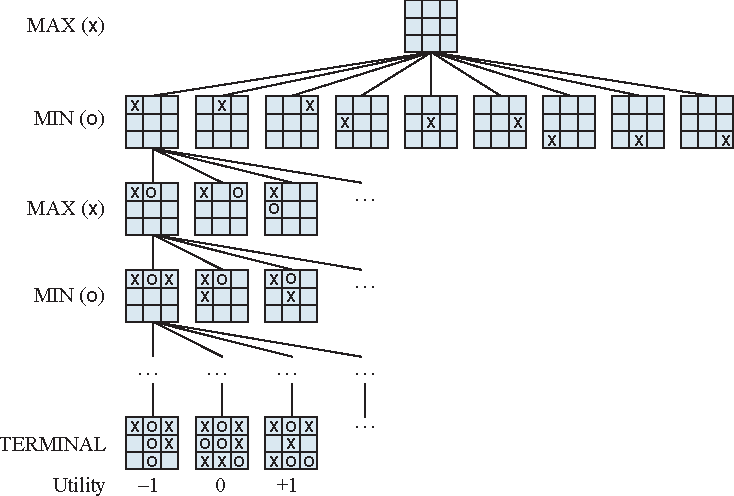
\includegraphics[scale=1.15]{Tic-Tac-Toe}
\caption{}\label{Tic-Tac-Toe}
\end{figure}
\subsection{Optimal decision: minimax}
In a normal search problem, the optimal solution would be a sequence of actions leading to a goal state—a terminal state that is a win. In adversarial search, MIN has something to say about it. MAX therefore must find a contingent \emph{strategy}.

Consider for instance the trivial game in Figure~\ref{Optimal_Decision}. The possible moves for MAX at the root node are labeled $a_1, a_2, a_3$. The possible replies to $a_1$ for MIN are $b_1, b_2, b_3$, and so on. The $\bigtriangleup$ nodes are ``MAX nodes'', in which it is MAX's turn to move, and the $\bigtriangledown$ nodes are ``MIN nodes''. This particular game ends after one move each by MAX and MIN. The utilities of the terminal states in this game range from 2 to 14. Given a game tree, the optimal strategy can be determined from the \textbf{minimax value} of each node. The minimax value of a node is the utility (for MAX) of being in the corresponding state, \emph{assuming that both players play optimally} from there to the end of the game. This means that MAX tries to maximize its yield, while MIN tries to minimize MAX's result\footnote{Put simply, each player tries to increase their yield, but sometimes it can be more useful to minimize that of the opponent (the two possibilities are not always interchangeable).}. Obviously, the minimax value of a terminal state is just its utility.
\begin{figure}[h!t]
\centering
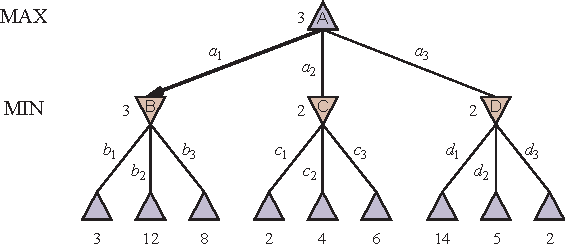
\includegraphics[scale=1.2]{Optimal Decision}
\caption{}\label{Optimal_Decision}
\end{figure}

In the particular case of Fig.~\ref{Optimal_Decision}, the first MIN node, labeled B, has three successor states with utility values 3, 12 and 8, so its minimax value is 3. In fact, if MAX reaches the node B and MIN plays at its best, then MAX will necessarily finish at the node with utility function 3. Similarly, the other two MIN nodes have minimax value 2. The root node is a MAX node; its successor states have minimax values 3, 2 and 2, so it has a minimax value of 3 (MAX's nodes always have the minimax value of the successor node with highest minimax value). We can also identify the \emph{minimax decision} at the root: action $a_1$ is the optimal choice for MAX because it leads to the state with the highest minimax value.

The minimax algorithm computes the minimax decision from the current state. It uses a simple recursive computation of the minimax values of each successor state, directly implementing the defining equations. The recursion proceeds all the way down to the leaves of the tree, and then the minimax values are \emph{backed up} through the tree as the recursion unwinds. For example, in Figure 5.2, the algorithm first recurses down to the three bottom-left nodes and uses the utility function on them to discover that their values are 3, 12 and 8, respectively. Then it takes the minimum of these values, 3, and returns it as the backed-up value of node B. A similar process gives the backed-up values of 2 for C and 2 for D.
\subsubsection{Multiplayer games}
Many popular games allow more than two players. Let us examine how to extend the minimax idea to multiplayer games. This is straightforward from the technical viewpoint, but raises some interesting new conceptual issues.

First, we need to replace the single value for each node with a vector of values. For example, in a three-player game with players A, B and C, a vector $(n_A,n_B,n_C)$ is associated with each node (Fig.~\ref{Multiplayer_Game}). For terminal states, this vector gives the utility of the state from each player's viewpoint (in two-player, zero-sum games, the two-element vector can be reduced to a single value because the values are always opposite).

Now we have to consider non-terminal states. Consider the node marked X in the game tree shown in Figure~\ref{Multiplayer_Game}. In that state, player C chooses what to do. The two choices lead to terminal states with utility vectors $(1,2,6)$ and $(4,2,3)$. Since 6 is bigger than 3, C should choose the first move. This means that if state X is reached, subsequent play will lead to a terminal state with utilities $(1,2,6)$. Hence, the backed-up value of X is this vector. The backed-up value of a node $n$ is always the utility vector of the successor state with the highest value for the player choosing at $n$.
\begin{figure}[h!t]
\centering
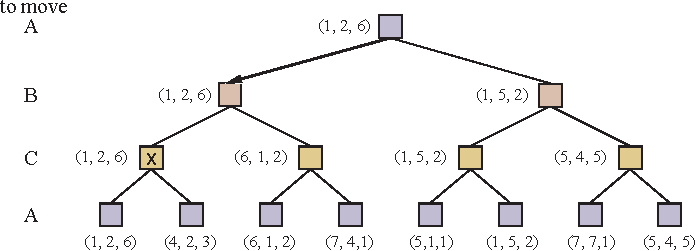
\includegraphics[scale=1.2]{Multiplayer Game}
\caption{}\label{Multiplayer_Game}
\end{figure}

Anyone who plays multiplayer games quickly becomes aware that much more is going on than in two-player games. Multiplayer games usually involve \emph{alliances}, whether formal or informal, among the players. Alliances are made and broken as the game proceeds. Alliances are still a natural consequence of optimal strategies for each player in a multiplayer game. For example, suppose A and B are in weak positions and C is in a stronger position. Then it is often optimal for both A and B to attack C rather than each other, lest C destroy each of them individually. In this way, collaboration emerges from purely selfish behavior. Of course, as soon as C weakens under the joint onslaught, the alliance loses its value, and either A or B could violate the agreement. So players must balance the immediate advantage of joining forces against the long-term advantage that other players can benefit.
\subsection{Alpha–beta pruning}
The problem with minimax search is that the number of game states it has to examine is exponential in the depth of the tree. Unfortunately, we can't eliminate the exponent, but it turns out we can effectively cut it in half. The trick is that it is possible to compute the correct minimax decision without looking at every node in the game tree. That is, we can borrow the idea of \emph{pruning} to eliminate large parts of the tree from consideration. The particular technique we examine is called \textbf{alpha–beta pruning}. When applied to a standard minimax tree, it returns the same move as minimax would, but prunes away branches that cannot possibly influence the final decision.

Alpha–beta pruning can be applied to trees of any depth, and it is often possible to prune entire subtrees rather than just leaves. The general principle is this: consider a node $n$ somewhere in the tree, such that the player at root has a choice of moving to that node. If that layer has a better choice $m$ either at the parent node of $n$ or at any choice point further up, then $n$ will never be reached in actual play. So once we have found out enough about $n$ (by examining some of its descendants) to reach this conclusion, we can prune it.

In practice let's consider the example of Figure~\ref{Alpha-Beta_Pruning}, showing the tages in the calculation of the optimal decision. At each point are shown the range of possible minimax values for each node. (a) We start by examining the deepest nodes of the tree; the first leaf below B has the utility value 3. Hence B, which is a MIN node, has a minimax value of \emph{at most} 3 (restricted to the interval $(-\infty,3]$). (b) The second leaf below B has a utility value of 12; MIN would avoid this move, so the value of B is still at most 3. (c) The third leaf below B has a value of 8, i.e. again larger than the other; we have seen all B's successor states, so we can conclude that the minimax value of B is exactly 3. Now, we can also infer that the value of the root is \emph{at least} 3, because MAX has a choice worth 3 at the root. (d) Let's now analyze the other branches. The first leaf below C has the value 2. Hence C, which is a MIN node, has a value of at most 2. But we know that B is worth 3, so MAX would never choose C. Therefore, there is no point in looking at the other successor states of C. This is an example of alpha–beta pruning. (e) The first leaf below D has the value 14, so D is worth at most 14. This is still higher than MAX's best alternative (i.e., 3), so we need to keep exploring D's successor states. Notice also that we now have bounds on all of the successors of the root, so the root's value is also at most 14. (f) The second successor of D is worth 5, so again we need to keep exploring. The third successor is worth 2, so now D is worth exactly 2. MAX's decision at the root is to move to B, giving a value of 3.
\begin{figure}[h!t]
\centering
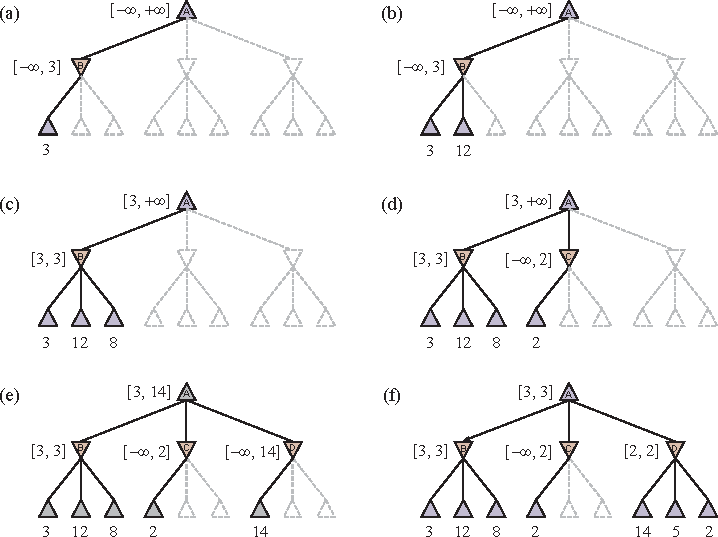
\includegraphics[width=\textwidth]{Alpha-Beta Pruning}
\caption{}\label{Alpha-Beta_Pruning}
\end{figure}

The effectiveness of alpha–beta pruning is highly dependent on the \emph{order} in which the states are examined. For example, in (e) and (f), we could not prune any successors of D at all because the worst successors (from the point of view of MIN) were generated first. If the third successor of D had been generated first, we would have been able to prune the other two. This suggests that it might be worthwhile to try to examine first the successors that are likely to be best. To do this, however, we need an a priori knowledge of the tree.
\subsection{Evaluation function}
The minimax algorithm generates the entire game search space, whereas the alpha–beta algorithm allows us to prune large parts of it. However, alpha–beta still has to search all the way to terminal states for at least a portion of the search space. This depth is usually not practical, because moves must be made in a reasonable amount of time—typically a few minutes at most. E.g., in chess is practically impossible to reach analytically the terminal state.

Claude Shannon's paper ``Programming a Computer for Playing Chess'' (1950) proposed instead that programs should cut off the search earlier and apply a heuristic \textbf{evaluation function} to states in the search, effectively turning non-terminal nodes into terminal leaves.
%In other words, the suggestion is to alter minimax or alpha–beta in two ways: replace the utility function by a heuristic evaluation function $\textsc{Eval}\s(s)$, which \emph{estimates} the position's utility, and replace the terminal test by a cutoff test that decides when to apply $\textsc{Eval}\s(s)$.
%in the previous sections, h was underestimating
An evaluation function returns an \emph{estimate} of the expected utility of the game from a given position, just as the heuristic functions of Chapter~\ref{chap:1} return an estimate of the distance to the goal.
%The idea of an estimator was not new when Shannon proposed it. For centuries, chess players have developed ways of judging the value of a position because humans are even more limited in the amount of search they can do than are computer programs.
How exactly do we design good evaluation functions?
\begin{itemize}
\item First, the evaluation function should order the terminal states in the same way as the true utility function: states that are wins must evaluate better than draws, which in turn must be better than losses. Otherwise, an agent using the evaluation function might err even if it can see ahead all the way to the end of the game.
\item Second, the computation must not take too long (the whole point is to search faster!).
\item Third, for non-terminal states, the evaluation function should be strongly correlated with the actual chances of winning.
\end{itemize}
One might well wonder about the phrase ``chances of winning''. After all, chess is not a game of chance, since we know the current state with certainty. But if the search must be cut off at non-terminal states, then the algorithm will necessarily be uncertain about the final outcomes of those states. This type of uncertainty is induced by computational, rather than informational, limitations. Given the limited amount of computation that the evaluation function is allowed to do for a given state, the best it can do is make a guess about the final outcome.

%One of the most immediate ways to estimate the evaluation function could be to study the typical outcome of the game as a function of pieces on the board. For example, suppose our experience suggests that \SI{72}{\percent} of the states encountered in the two-pawns vs. one-pawn category lead to a win (utility $+1$), \SI{20}{\percent} to a loss ($-1$) and \SI{8}{\percent} to a draw ($0$). Then a reasonable evaluation for states in the category is the weighted average of the values, also called expected value: $0.72\cdot1-0.20\cdot1+0.08\cdot0=0.52$. In principle, the expected value can be determined for each category, i.e. for different combinations of pieces, resulting in an evaluation function that works for any state.
Most evaluation functions work by calculating various \emph{features} of the state—for example, in chess, we would have features for the number of white pawns, black pawns, white queens, black queens, and so on. The features, taken together, define various \emph{categories} or equivalence classes of states: the states in each category have the same values for all the features. For example, one category contains all two-pawn vs. one-pawn endgames. Any given category, generally speaking, will contain some states (position of those pieces) that lead to wins, some that lead to draws and some that lead to losses. The evaluation function cannot know which states are which, but it can return a single value that reflects the proportion of states with each outcome. For example, suppose our experience suggests that \SI{72}{\percent} of the states encountered in the two-pawns vs. one-pawn category lead to a win (utility $+1$), \SI{20}{\percent} to a loss ($-1$) and \SI{2}{\percent} to a draw ($0$). Then a reasonable evaluation for states in the category is the weighted average of the values (also called expected value). In principle, the expected value can be determined for each category, resulting in an evaluation function that works for any state.

In practice, this kind of analysis requires too many categories and hence too much experience to estimate all the probabilities of winning. Instead, most evaluation functions compute separate numerical contributions from each feature and then combine them to find the total value. For example, introductory chess books give an approximate ``material value'' for each piece: each pawn is worth 1, a knight or bishop is worth 3, a rook 5 and the queen 9. Other features such as ``good pawn structure'' and ``king safety'' might be worth half a pawn, say. These feature values are then simply added up to obtain the evaluation of the position. Mathematically, this kind of evaluation function is essentially a weighted linear combination, because it can be expressed as
\begin{equation}
\textsc{Eval}\s(s)=w_1f_1(s)+w_2f_2(s)+\ldots+w_nf_n(s)=\sum_{i=1}^nw_if_i(s)
\end{equation}
where each $w_i$ is a weight and each $f_i$ is a feature of the position. For chess, the $f_i$ could be the numbers of each kind of piece on the board, and the $w_i$ could be the values of the pieces (1 for pawn, 3 for bishop, etc.). The weights aren't necessarily constant; they are application coefficients that can vary with stage of game (opening, middle game, endgame), pieces on the board (e.g. presence or absence of queens), other characteristics of the position, or high level strategy or plans.

%two pawn in columns is not good, etc.
The astute reader will have noticed that the features and weights are not part of the rules of chess! They come from centuries of human chess-playing experience. It should be clear that \emph{the performance of a game-playing program depends strongly on the quality of its evaluation function}. An inaccurate evaluation function will guide an agent toward positions that turn out to be lost. 
\subsubsection{Horizon effect}
The idea of an evaluation function is very powerful in reducing the search tree, but in some particular cases, the fact of having cut the search tree can cause problems. An intuitive example is so-called \textbf{horizon effect}, that arises when the program is facing an opponent's move that causes serious damage and is ultimately unavoidable, but can be temporarily avoided by delaying tactics.

Consider for instance the chess state depicted in Figure~\ref{Horizon_Effect}, in which is the turn of Black to move. By moving in a1 the black rook can actually check the white king. However, in response the king can move one position diagonally (in g2) to get out of check. The rook can then repeat the check by moving in a2, but in turn the king can once again delay the defeat by moving diagonally (in f1). One may therefore wonder which of the two sides is advantaged. This configuration is in whose favor?
\begin{figure}[ht]
\centering
\setlength{\fboxsep}{0.08em+0.045em+0.08em}
\setlength{\fboxrule}{0pt}
\def\mylabelleftformat{\setlength{\fboxsep}{0pt}\makebox[0pt][r]{\arabic{ranklabel}}}
\fcolorbox{black}{white}{%
\setboardfontcolors{blackfieldmask=gray!30}
\setchessboard{%
showmover=true,
mover=b,
marginrightwidth=7.3mm,
marginleftwidth=2.27mm,%+0.4mm
margintopwidth=0em,
marginbottomwidth=4.64mm,%+0.3mm
borderwidth=0.04em,
linewidth=0.04em,
pgfborder,
padding=0.09em,
pgfborder,
labelleftwidth=2.651mm,%+0.4mm  %{1.861mm-0.104mm+0.08em}
labelbottomlift=4.692mm,%+0.3mm  %{3.9mm+0.492mm}
setpieces={Kh1,Ph3,Pg3,Pf3,Pe3,Pd3,Pd7,ra2,ka6,pc6,pb7,pf7,pg7,ph7},
boardfontencoding=LSBC4,
setfontcolors,
labelleftformat=\mylabelleftformat,
pgfstyle=straightmove,
linewidth=1.0pt,
color=gray!90,
shortenstart=+0.875ex,
markmoves={h1-g2},
shortenstart=+0.0ex,
markmoves={g2-f1,f1-e2,e2-d1,d1-c2},
%pgfstyle=curvemove,
%markmoves={a2-a1,a1-a2},
}
\newgame
\chessboard}
\caption{}\label{Horizon_Effect}
\end{figure}

It is clear that the line made up of white pawns is trapping the king under the influence of the rook. However, a human player would understand that the block is actually temporary, since after some zigzagging the king can in reality escape the block and move with freedom across all the board, with the possibility to exploit also the other pieces. In particular, the white pawn in d7 may be easily promoted to a queen, giving a huge advantage to White and securing the king. Thus, a human player would claim that White is currently in the lead.

Instead, the evaluation of a computer might be different, depending on the depth of the search. For instance, if the algorithm stops analyzing the search tree only after 3 moves from the state of Figure~\ref{Horizon_Effect}, then it will say that Black is in the lead because it has a rook and the opponent only pawns. On the other hand, if the algorithm is implemented sufficiently in depth to explore many more moves, i.e. to see over the horizon, then it will notice that the pawn might become a queen, giving an important jump in the evaluation function for White.
In other words, a series of checks by the black rooks forces the inevitable queening move by White ``over the horizon'' and makes this position look like a win for Black, when it is really a win for White.

This horizon effect is inherent in adopting a truncated search tree and cannot be eliminated, but it can still be mitigated (e.g., by introducing exceptions in the algorithm that allow specific solving moves for specific configurations leading to the horizon effect). This effect is even more emphasized in the game of Go because of the presence of larger structures, where the algorithm would be forced to look more than 10 moves forward to see right.
\subsection{Monte Carlo tree search}
Another very powerful technique to study board games is \textbf{Monte Carlo tree search} (MCTS), which in some sense computes an evaluation function in an automatic way. Its purpose is to analyze the most promising moves by expanding the search tree based on random sampling of the search space. The application of Monte Carlo tree search in games is based on many \emph{playouts}, also called \emph{roll-outs}. In each playout, the game is played out to the very end by selecting moves at random. The final game result of each playout is then used to weight the nodes in the game tree so that better nodes are more likely to be chosen in future playouts.

The algorithm is organized in four steps:
\begin{itemize}
\item Selection: Starting from the root node $R$ of the search tree, we go down the tree by repeatedly selecting legal moves until we reach a leaf node $L$. Recall that the root is the current game state (from which we must take an optimal decision) and a leaf is any node that has a potential child from which no simulation (playout) has yet been initiated. So if one, several or all of the legal moves in a node does not have a corresponding node in the search tree, we stop selection. We will return on how to efficiently choose the path later on (see below).
%walking across the nodes with the highest winning probability. 
\item Expansion: Unless $L$ ends the game decisively for either player (e.g. win/loss/draw), create its possible child nodes, which are any available action from the game position defined by $L$ (i.e. expand it). Then choose to explore node $C$ from one of them.
\item Simulation: Starting from the newly-created node in the expansion phase, let's complete one random playout by selecting randomly each move till the end. As said before, a playout may be as simple as choosing uniform random moves until the game is decided (for example in chess, the game is won, lost or drawn). No new nodes are created in this phase.
%This step is sometimes also called playout or rollout. 
\item Backpropagation: Once a winner has emerged from the simulation phase, use the result of the playout to update information in the nodes on the path from $C$ to $R$. Each visited node has its simulation count (the denominator) incremented, while its win count may also be incremented, depending on which player wins.
\end{itemize}
Refer for instance to Figure~\ref{Monte_Carlo_Tree_Search}. This graph shows the steps involved in one decision (i.e. one move in the real world), with each node presenting the ratio of wins to total playouts from that point in the game tree for the player that the node represents. For example, the root node says there are 12 wins out of 21 playouts for White from this position so far.
%It complements the total of $9/21$ Black wins shown along the three black nodes under it, each of which represents a possible black move.
Once chosen a path till a leaf node (shown in bold), we choose one of its possible child nodes; we initialize it with the ratio $0/0$. At this point we start a new random game from that specific node and depending on the outcome we consequently update the numbers of the nodes along the chosen path. For instance, if White loses the simulation, all nodes along the selection incremented their simulation count (the denominator), but among them only the black nodes were credited with wins (the numerator). If instead White wins, all nodes along the selection would still increment their simulation count, but among them only the white nodes would be credited with wins. In games where draws are possible, a draw causes the numerator for both black and white to be incremented by 0.5 and the denominator by 1.
\begin{figure}[h!t]
\centering
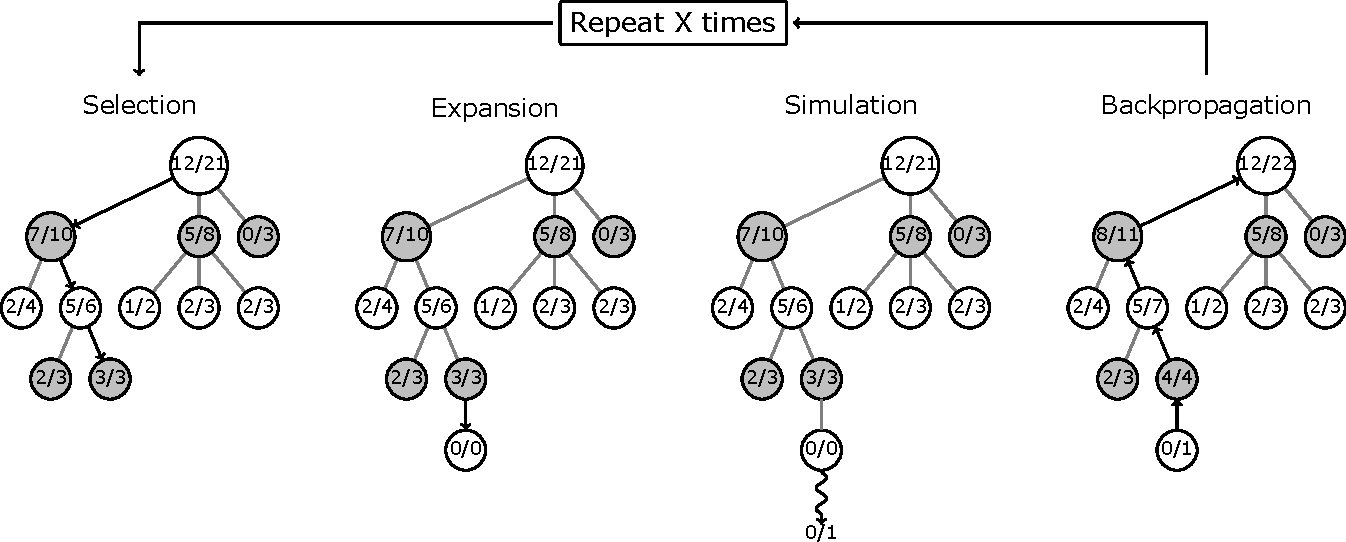
\includegraphics[width=\textwidth]{Monte Carlo Tree Search (Modified)}
\caption{}\label{Monte_Carlo_Tree_Search}
\end{figure}

As we have previously anticipated, the choice of the path in the first step can severely affect the efficiency of the algorithm, and therefore the proposition of an optimal move. Our path selection should achieve two goals: we should \emph{explore} new paths to gain information on as many moves as possible, and we should also use existing information to \emph{exploit} paths known to be good (i.e. giving a high win rate). In order to help us achieve these two goals, we need to select child nodes using a selection function that balances exploration and exploitation. One (bad) way to do this is to select paths randomly. Random selection certainly does explore well, but it does not exploit at all. Another (equally bad) way is to use the average win rate of each node. This achieves good exploitation, but it scores poorly on exploration. Luckily, some very smart people have figured out a good selection function that balances exploration with exploitation well, called UCB1 (Upper Confidence Bound 1). When applied to MCTS, the combined algorithm is named UCT (Upper Confidence bound 1 applied to Trees). So, $\text{MCTS}+\text{UCB1}=\text{UCT}$. The UCB1 selection function is given by
\begin{equation}
\frac{w_i}{n_i}+c\sqrt{\frac{\ln{s_p}}{n_i}}
\end{equation}
where
\begin{itemize}
\item $w_i$ is the number of simulations that result in a win for the considered node after the $i$-th move;
\item $n_i$ is the number of simulations for the considered node after the $i$-th move;
\item $s_p$ is the total number of simulations after the $i$-th move run by the parent node of the one considered;
\item $c$ is the exploration parameter, in practice usually chosen empirically.
\end{itemize}
The left term is the \emph{exploitation} term. It is simply the average win rate, going larger the better a node has historically performed. The right term is the exploration term. It goes larger the less frequently a node is selected for simulation. The exploration parameter $c$ is just a number we can choose that allows us to control how much the equation favors exploration over exploitation. Note that the numbers inside the nodes in the tree diagram of Figure~\ref{Monte_Carlo_Tree_Search} are the statistics for that node, corresponding to number of wins and total number of simulations ($w_i$ and $s_i$). Each time we need to select a path across multiple nodes, we use the UCB1 selection function to get a value for each child node, and we select the child node with the \emph{maximum} value. This also means that the selected path may not be the same after each round, i.e. after a sequence of these four steps, because the update taking place in the ``Backpropagation'' can modify the hierarchy of UCB1 values in the tree. So, MCTS does not need an explicit evaluation function; simply implementing the game's mechanics is sufficient to explore the search space.

In summary, during one round of search the path is selected according to the right balance between win rate and exploration frequency. Then, rounds of search are repeated as long as the time allotted to a move in the real world is respected. The efficiency of this method often increases with time as more playouts are assigned to the moves that have frequently resulted in the current player's victory according to previous playouts. Finally, only the \emph{move with the most simulations made} (i.e. the highest denominator) is chosen as the final answer, that is in the ``training'' we evaluate the possible moves according to UCB1, but the ultimate choice falls on the move that has seen the greatest number of simulations.
%How we implement the very beginning, in which R=L? Before choosing C we have to evaluate the possible children; but these must be drawn on the tree (and set to 0/0), or only determined and drawn just the C chosen? In the former case, however, we don't know how to deal with UCB1=0/0 and the picture should be modified (?), whereas in the latter we would have only one possible path always.
%---------------------------------------------------------------------------------------------------------------------------------------------------
%https://en.wikipedia.org/wiki/Monte_Carlo_tree_search
%https://medium.com/@quasimik/monte-carlo-tree-search-applied-to-letterpress-34f41c86e238
%https://www.analyticsvidhya.com/blog/2019/01/monte-carlo-tree-search-introduction-algorithm-deepmind-alphago/
























